% ch3-legendre.tex
\documentclass[../main/main]{subfiles}

\begin{document}
\small



\chapter{Legendre関数}

\vspace{-180pt}
\begin{figure}[H]
  \begin{flushright}
    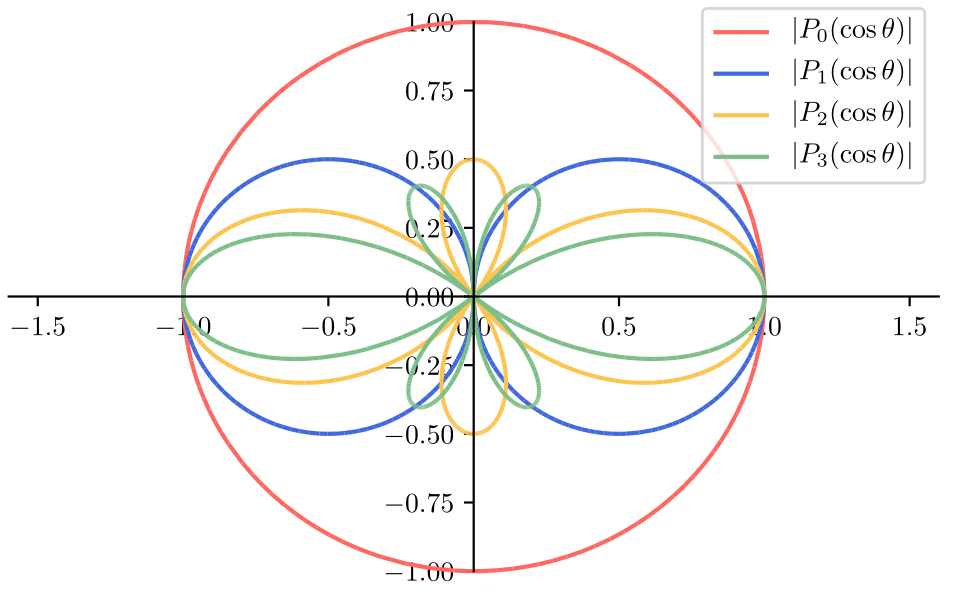
\includegraphics[width=90mm]{../fig/legendre/legendre_title.png}
  \end{flushright}
\end{figure}

\vspace{-12pt}
\footnotesize
Legendre関数は球対称な系の偏微分方程式を考える際に
必ずといってよいほど解として現れる関数である。
たとえばLaplace方程式$\Delta \psi = 0$を球座標系$(r, \theta, \varphi)$で変数分離すると
天頂角$\theta$成分については
\begin{equation}\label{eq:legendre-diff}
  \[ \frac{1}{\sin\theta} \frac{d}{d\theta} \( \sin\theta \frac{d}{d\theta} \)
	+ \left\{ l(l+1) - \frac{m^2}{\sin^2\theta} \right\} \] y = 0
\end{equation}
なる方程式が現れ、解は(第1種)Legendre陪関数$P_m^l(x)$によって記述される。
そしてLegendre陪関数が満たす各性質はLegendre多項式$P_n(x)$の性質から導かれる。
またLegendre多項式$P_n(x)$は微分方程式の解として以外にもさまざまな応用例がある。
多くの場合、整数次のLegendre関数$P_n(x), \ P_m^l(x)$のみが問題となるため、
本稿においてはこれらの関数の性質を調べるにとどめ、
一般次数のLegendre関数$P_\nu^\mu(x)$や
\eqref{eq:legendre-diff}の第二の解として現れる第2種Legendre関数$Q_\nu^\mu(x)$については
扱わないことにする。


\small
\section{Legendre多項式}
\subsection{Legendre多項式}
Legendre多項式$P_n(x)$は区間$[-1, 1]$で定義される直交多項式である。
これまでの特殊関数と同様、Legendre多項式も母関数\eqref{eq:Pn-gene}によって定義するのが便利である。
最もよく知られた性質はRodriguesの公式\eqref{eq:Pn-Rod}であろう。
Legendre多項式の漸化式は他の特殊関数と趣きが異なり、構造が多少複雑になっている。
そのためもあってか$P_n(x)$が満たす漸化式は数多く作ることができる。
実際によく使われるのは\eqref{eq:Pn-req-3ko}くらいであろうが、
導出過程を簡明にするためあえて数多くの漸化式を載せてある。
すべての漸化式を覚えねばならないと気を張る必要はない。
微分方程式は\eqref{eq:Pn-diff-req-2k0-2}と\eqref{eq:Pn-kako}の微分から
$P_{n-1}^\prime (x)$を消去することで導く教科書が多く、それに処理量も少なくて済むのであるが、
本稿ではこれまで通り昇降演算子を用いた導出手法を載せることにした。
やや計算量が多くなってしまうが、確実に目標の式にたどり着けるという安心感はある。
Legendre多項式に関する公式の導出過程は少し巧妙な部分が多いので、
注意深く式展開を追っていきたい。


\subsubsection*{公式集}

\paragraph{母関数(定義)}
\begin{equation}\label{eq:Pn-gene}
  g(t, x) = \frac{1}{\sqrt{1-2xt+t^2}} 
		= \sum_{n=0}^\infty P_n(x) t^n
		\qquad (|t|<1)
\end{equation}

\paragraph{偶奇性}
\begin{equation}
  P_n(-x) = (-1)^n P_n(x)
\end{equation}

\paragraph{$x=0$での特殊値}
\begin{subnumcases}{}
  P_{2n} (0) = (-1)^n \frac{(2n-1)!!}{(2n)!!} & \label{eq:Pn-x=0-1}\\
  P_{2n+1} (0) = 0 & \label{eq:Pn-x=0-2}
\end{subnumcases}

\paragraph{$x=\pm1$での特殊値}
\begin{subnumcases}{}
  P_n(1) = 1 & \label{eq:Pn-x=1}\\
  P_n(-1) = (-1)^n & \label{eq:Pn-x=-1}
\end{subnumcases}

\paragraph{一般項}
\begin{equation}\label{eq:Pn-ippan}
  P_n(x) = \sum_{i=0}^{\lfloor \frac{n}{2} \rfloor} \frac{(-1)^i (2n-2i)!}{2^n\,  i!\, (n-i)! (n-2i)! }x^{n-2i}
\end{equation}

\paragraph{Rodriguesの公式}
\begin{equation}\label{eq:Pn-Rod}
  P_n(x) = \frac{1}{2^n n!} \dx{n} (x^2-1)^n
\end{equation}

\paragraph{漸化式(3項間)}
\begin{equation}\label{eq:Pn-req-3ko}
  (2n+1) x P_n(x) = n P_{n-1}(x) + (n+1) P_{n+1} (x)
\end{equation}

\paragraph{微分漸化式(3項間)}
\begin{equation}\label{eq;Pn-diff-req-3ko}
  2x P_n^\prime(x) + P_n(x) = P_{n-1}^\prime (x) + P_{n+1}^\prime (x)
\end{equation}

\paragraph{微分漸化式(2項間)}
\begin{align}
  &(n+1) P_n(x) + x P_n^\prime(x) = P_{n+1}^\prime (x) \label{eq:Pn-diff-req-2k0-1}\\
  &n P_n(x) - x P_n^\prime (x) = -P_{n-1}^\prime (x) \label{eq:Pn-diff-req-2k0-2}
\end{align}


\paragraph{微分漸化式(3項間)II}
\begin{equation}\label{eq:Pn-diff-req-3ko-II}
  (2n+1) P_n(x) = -P_{n-1}^\prime (x) + P_{n+1}^\prime (x) 
\end{equation}

\paragraph{昇降演算子}
\begin{alignat}{2}
  &\textbf{下降演算子} &\qquad  &  \[ (1-x^2)\dx{} + nx \] P_n(x) = n P_{n-1} (x) \label{eq:Pn-kako}\\
  &\textbf{上昇演算子} & & \[ (1-x^2) \dx{} - (n+1)x \] P_n(x) = -(n+1) P_{n+1} (x) \label{eq:Pn-josho}
\end{alignat}

\paragraph{微分方程式}
\begin{equation}
  (1-x^2) \frac{d^2 P_n(x)}{dx^2} - 2x \frac{d P_n(x)}{dx} + n(n+1) P_n(x) = 0
\end{equation}

\paragraph{自己随伴形}
\begin{equation}
  \dx{} \[ (1-x^2) \dx{} P_n(x) \] + n(n+1) P_n(x) = 0
\end{equation}

\paragraph{直交性}
\begin{equation}\label{eq:Pn-choko}
  \int_{-1}^1 P_m(x) P_n(x) dx = \frac{2}{2n+1} \delta_{mn}
\end{equation}

\vspace{-12pt}
\begin{figure}[bt]
\begin{tabular}{cc}
 \begin{minipage}{0.40\hsize}\small
    \begin{table}[H]
      \centering
      \small
      \caption{Legendre多項式$P_n(x)$}
      \begin{tabular}{l}\Hline
        $P_0(x) \ = \ 1$ \\
        $P_1(x) \ = \ x$ \\
        $P_2(x) \ = \ \frac{1}{2} (3x^2-1)$ \\
        $P_3(x) \ = \ \frac{1}{2} (5x^3-3x)$ \\
        $P_4(x) \ = \ \frac{1}{8} (35x^4 - 30x^2 + 3)$ \\
        $P_5(x) \ = \ \frac{1}{8} (63x^5 - 70x^3 + 15x)$ \\
        $P_6(x) \ = \ \frac{1}{16} (231x^6 - 315x^4 + 105x^2- 5 )$ \\\hline
      \end{tabular}
    \end{table}
 \end{minipage}

\hspace{-2pt}
 \begin{minipage}{0.60\hsize}
    \begin{figure}[H]
      \centering
      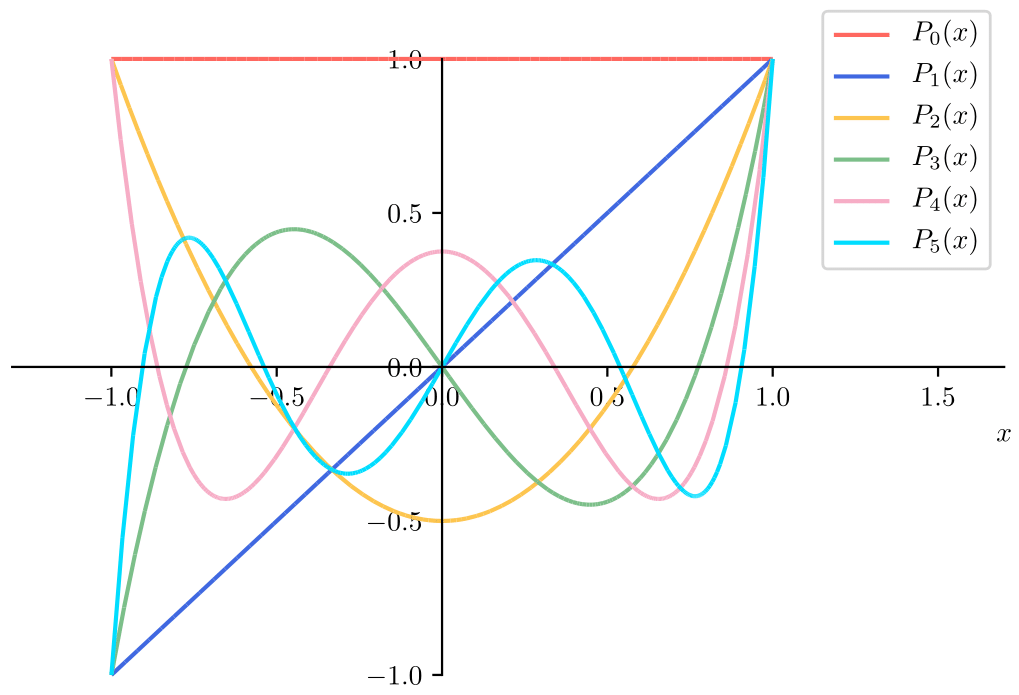
\includegraphics[width=	80mm]{../fig/legendre/legendre.png}
      \caption{Legendre多項式 \ $P_n(x)$}
    \end{figure}
  \end{minipage}
\end{tabular}
\end{figure}

\subsubsection*{証明}

\paragraph{母関数 $\Longrightarrow$ 偶奇性}
母関数\eqref{eq:Pn-gene}の中辺から$g(-t, -x) = g(t, x)$が成立することが分かるので、
\eqref{eq:Pn-gene}の右辺から
\begin{equation*}
  \sum_{n=0}^\infty P_n(-x) \ (-t)^n 
	\sum_{n=0}^\infty P_n(x) t^n
\end{equation*}
$t^n \ (n\geq 0)$の係数を比較して、
\begin{equation*}
  P_n(-x) = (-1)^n P_n(x)
\end{equation*}\qed

\paragraph{母関数 $\Longrightarrow$ $x=0$での特殊値}
母関数\eqref{eq:Pn-gene}に$x=0$を代入すると、
\begin{equation}\label{eq:Ln-gene->x=0-En}
  g(t, 0) = \frac{1}{\sqrt{1+t^2}} 
		= \sum_{n=0}^\infty P_n(0) t^n
\end{equation}
ここで\eqref{eq:Ln-gene->x=0-En}の中辺は$\frac{1}{\sqrt{1-t}}$の展開公式\eqref{eq:1/sqrt(1-t)}
\footnote{
\begin{equation}\label{eq:1/sqrt(1-t)}
  \frac{1}{\sqrt{1-t}} = \sum_{n=0}^\infty \frac{(2n)!}{2^{2n} (n!)^2} t^n
	= \sum_{n=0}^\infty \frac{(2n-1)!!}{(2n)!!} t^n
	\qquad (|t|<1)
\end{equation}
証明には二項展開を行えばよい。
\begin{align*}
  \frac{1}{\sqrt{1-t}} &= (1-t)^{-\frac{1}{2}}
	= \sum_{n=0}^\infty \binom{-\frac{1}{2}}{n} (-t)^n
	= \sum_{n=0}^\infty \frac{\( -\frac{1}{2} \)\( -\frac{3}{2} \)\dots \( -\frac{1}{2} - n + 1 \)}{n!} (-t)^n\\
	&= \sum_{n=0}^\infty \frac{1\cdot 3 \dots (2n-1)}{2^n n!} t^n
	= \sum_{n=0}^\infty \frac{(2n-1)!!}{(2n)!!} t^n
	= \sum_{n=0}^\infty \frac{(2n)!}{2^{2n} (n!)^2} t^n
\end{align*}
\qed

\noindent ここで二重階乗についての以下の関係を用いている。
\begin{equation}
  (2n)!! = 2^n n! , \qquad (2n-1)!! = \frac{(2n)!}{(2n)!!} = \frac{(2n)!!}{2^n n! }
\end{equation}
\eqref{eq:1/sqrt(1-t)}は非常に重要であり、記憶に値する。
}
において$t$を$-t^2$に置き換えることで
\begin{equation*}
  \frac{1}{\sqrt{1+t^2}} 
	= \sum_{n=0}^\infty \frac{(2n-1)!!}{(2n)!!} (-t^2)^{n} 
	= \sum_{n=0}^\infty (-1)^{n} \frac{(2n-1)!!}{(2n)!!} t^{2n} 
\end{equation*}
一方\eqref{eq:Ln-gene->x=0-En}の右辺は
\begin{equation*}
  \sum_{n=0}^\infty P_n(0) t^n
	= \sum_{n=0}^\infty P_{2n}(0) t^{2n} + \sum_{n=0}^\infty P_{2n+1}(0) t^{2n+1}
\end{equation*}
と分解できる。
よって$t^n \ (n \geq 0)$の係数を比較して\eqref{eq:Pn-x=0-1}, \eqref{eq:Pn-x=0-2}を得る。\qed

\vspace{10pt}
\paragraph{母関数 $\Longrightarrow$ $x=\pm 1$での特殊値}
母関数\eqref{eq:Pn-gene}に$x=\pm 1$を代入すると、
\begin{equation}
  g(t, \pm 1) = \frac{1}{\sqrt{1\mp 2t+t^2}} 
		= \sum_{n=0}^\infty P_n(\pm 1) \, t^n
\end{equation}
中辺は等比級数の和の公式から
\begin{equation*}
  \frac{1}{\sqrt{1\mp 2t+t^2}} 
	= \frac{1}{1\mp t}
	= \sum_{n=0}^\infty (\pm t)^n
	= \sum_{n=0}^\infty (\pm 1)^n t^n
\end{equation*}
となるので、
右辺と$t^n \ (n \geq 0)$の係数を比較して\eqref{eq:Pn-x=1}, \eqref{eq:Pn-x=-1}を得る。\qed

\vspace{10pt}
\paragraph{母関数 $\Longrightarrow$ 一般項}
母関数\eqref{eq:Pn-gene}の中辺を公式\eqref{eq:1/sqrt(1-t)}を用いて展開すると、
\begin{equation*}
  g(t, x)
	= \frac{1}{\sqrt{1-(2xt-t^2)}} 
	= \sum_{m=0}^\infty \frac{(2m)!}{2^{2m} (m!)^2} (2xt-t^2)^m
\end{equation*}
ここで二項定理により
\begin{equation*}
  (2xt-t^2)^m = t^m (2x-t)^m
	= t^m \sum_{i=0}^m \binom{m}{i} (2x)^{m-i} (-t)^i 
	= \sum_{i=0}^m \frac{(-1)^i m!}{i! \, (m-i)!} (2x)^{m-i} t^{m+i}
\end{equation*}
であるから、
\begin{align}
  g(t, x)
	&= \sum_{m=0}^\infty \frac{(2m)!}{2^{2m} (m!)^2} 
		\sum_{i=0}^m \frac{(-1)^i m!}{i! \, (m-i)!} (2x)^{m-i} t^{m+i} \notag\\
	&= \sum_{m=0}^\infty \sum_{i=0}^m \frac{(-1)^i (2m)!}{2^{m+i} \, i! \, m! (m-i)!} x^{m-i} t^{m+i}
		\label{eq:Pn-gene->ippan}
\end{align}

\vspace{-12pt}
\begin{figure}[H]
  \begin{tabular}{c}
 \begin{minipage}{0.54\hsize}\small
ここで$m+i$を新たに$n$と置き換えて$m, i$についての二重和を$n, i$についての二重和に取りかえる。
$m$について$0$から$\infty$まで、$i$について$0$から$m$まで加えていくとき、
二重和は図\ref{fig:legendre}の黒丸で表した格子点すべてについて実行される。
$n=m+i$であるとき、$n=0, 1, 2, \dots$に対応する全格子点は
図\ref{fig:legendre}で示した各直線上の点として捉えることができる。
したがって図\ref{fig:legendre}より、\eqref{eq:Pn-gene->ippan}における二重和は、
$n$について$0$から$\infty$まで、$i$について$0$から$\lfloor \frac{n}{2} \rfloor$までの二重和に
取りかえられることになる。ただし$\lfloor \frac{n}{2} \rfloor$とは
$\frac{n}{2}$を超えない最大の整数を意味する。よって、
 \end{minipage}
  
  \begin{minipage}{0.04\hsize}
    \hspace{0pt}
  \end{minipage}

 \begin{minipage}{0.42\hsize}
    \centering
    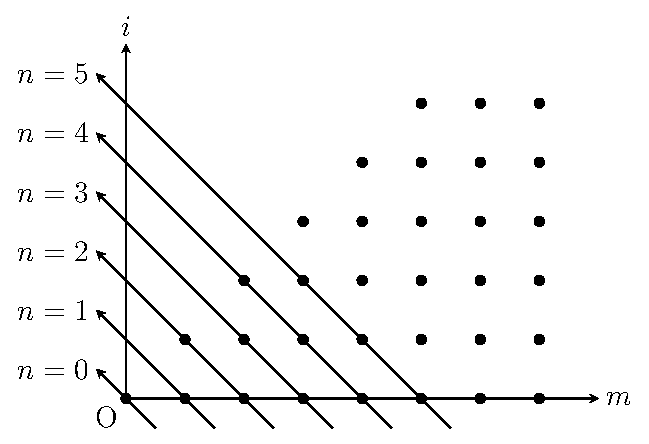
\includegraphics[width=60mm]{../TikZ/legendre/legendre.pdf}
    \caption{二重和の取りかえ方}
    \label{fig:legendre}
 \end{minipage}
  \end{tabular}
\end{figure}

\vspace{-12pt}
\begin{equation*}
  g(t, x) 
	= \sum_{n=0}^\infty \sum_{i=0}^{\lfloor \frac{n}{2} \rfloor} 
		\frac{(-1)^i (2n-2i)!}{2^{n} \, i! \, (n-i)! (n-2i)!} x^{n-2i} t^{n}
\end{equation*}
母関数\eqref{eq:Pn-gene}の右辺と比較して
\begin{equation*}
  P_n(x) = \sum_{i=0}^{\lfloor \frac{n}{2} \rfloor} \frac{(-1)^i (2n-2i)!}{2^n\,  i!\, (n-i)! (n-2i)! }x^{n-2i}
\end{equation*}\qed


\paragraph{一般項 $\Longrightarrow$ Rodriguesの公式}
一般項\eqref{eq:Pn-ippan}に対して
\begin{equation*}
  \dx{n} x^{2n-2i} = \frac{(2n-2i)!}{(n-2i)!}x^{n-2i}
\end{equation*}
であることを用いると、
\begin{align*}
  P_n(x) &= \sum_{i=0}^{\lfloor \frac{n}{2} \rfloor} \frac{(-1)^i }{2^n\,  i!\, (n-i)!} \cdot 
		\frac{(2n-2i)!}{(n-2i)!}x^{n-2i}
	= \sum_{i=0}^{\lfloor \frac{n}{2} \rfloor} \frac{(-1)^i }{2^n\,  i!\, (n-i)!} \dx{n} x^{2n-2i} \notag\\
	&= \frac{1}{2^n n!} \dx{n} \sum_{i=0}^{\lfloor \frac{n}{2} \rfloor} \frac{n!}{i!\, (n-i)!} (x^2)^{n-i} (-1)^i
		\notag\\
	&= \frac{1}{2^n n!} \dx{n} \sum_{i=0}^{\lfloor \frac{n}{2} \rfloor} \binom{n}{i} (x^2)^{n-i} (-1)^i
\end{align*}
ここで$\frac{n}{2} < i \leq n$のとき、$x$についての$n$階微分により$(x^2)^{n-i}$が$0$になるため、
これを新たに和に加えても差し支えない。すなわち、
\begin{align*}
  P_n(x) &=  \frac{1}{2^n n!} \dx{n} \sum_{i=0}^{n} \binom{n}{i} (x^2)^{n-i} (-1)^i \notag\\
	&= \frac{1}{2^n n!} \dx{n} (x^2-1)^n
\end{align*}\qed


\paragraph{母関数 $\Longrightarrow$ 漸化式(3項間)}
母関数\eqref{eq:Pn-gene}の中辺を$t$で偏微分することで
\begin{equation}\label{eq:Pn-gene->req}
  \frac{\6 g(t, x)}{\6 t} = \frac{x-t}{1-2xt+t^2} \, g(t, x)  \quad \iff \quad 
	 (1-2xt+t^2) \frac{\6 g(t, x)}{\6 t} = (x-t) \, g(t, x) 
\end{equation}
が成立することが分かる。いま、母関数\eqref{eq:Pn-gene}の右辺から
\begin{equation*}
  \frac{\6 g(t, x)}{\6 t}
	= \sum_{n=1}^\infty n P_n(x) t^{n-1}
	= \sum_{n=0}^\infty (n+1) P_{n+1} (x) t^n
\end{equation*}
であるので、これと母関数\eqref{eq:Pn-gene}の右辺を\eqref{eq:Pn-gene->req}に代入して
\begin{gather*}
   (1-2xt+t^2)  \sum_{n=0}^\infty (n+1) P_{n+1} (x) t^n
	= (x-t) \sum_{n=0}^\infty P_n(x) t^n \notag\\
  \sum_{n=0}^\infty (n+1) P_{n+1} (x) t^n - 2x\sum_{n=0}^\infty (n+1) P_{n+1} (x) t^{n+1}
		+ \sum_{n=0}^\infty (n+1) P_{n+1} (x) t^{n+2}
	= x\sum_{n=0}^\infty P_n(x) t^n - \sum_{n=0}^\infty P_n(x) t^{n+1}
\end{gather*}
$t$の指数をそろえると
\begin{gather*}
  \sum_{n=0}^\infty (n+1) P_{n+1} (x) t^n 
		- 2x\sum_{n=0}^\infty n P_{n} (x) t^{n}
		+ \sum_{n=0}^\infty (n-1) P_{n-1} (x) t^{n}
	= x\sum_{n=0}^\infty P_n(x) t^n 
		- \sum_{n=0}^\infty P_{n-1}(x) t^{n} \notag\\ \therefore \ 
  \sum_{n=0}^\infty 
	\[ (n+1)P_{n+1}(x) - (2n+1)x P_n(x) + n P_{n-1}(x) \] t^n = 0
\end{gather*}
$t^n \ (n \geq 0)$の係数を比較して次を得る。
\begin{equation*}
  (2n+1) x P_n(x) = n P_{n-1}(x) + (n+1) P_{n+1} (x)
\end{equation*}\qed

\paragraph{母関数 $\Longrightarrow$ 微分漸化式(3項間)}
母関数\eqref{eq:Pn-gene}の中辺を$x$で偏微分することで
\begin{equation}\label{eq:Pn-gene->diff-req}
  \frac{\6 g(t, x)}{\6 x} = \frac{t}{1-2xt+t^2} \, g(t, x)  \quad \iff \quad 
	 (1-2xt+t^2) \frac{\6 g(t, x)}{\6 x} = t \, g(t, x) 
\end{equation}
が成立することが分かる。いま、母関数\eqref{eq:Pn-gene}の右辺から
\begin{equation*}
  \frac{\6 g(t, x)}{\6 x}
	= \sum_{n=0}^\infty P_n^\prime(x) t^{n}
\end{equation*}
であるので、これと母関数\eqref{eq:Pn-gene}の右辺を\eqref{eq:Pn-gene->diff-req}に代入して
\begin{gather*}
  (1-2xt+t^2) \sum_{n=0}^\infty P_n^\prime(x) t^{n}
	= t \sum_{n=0}^\infty P_n(x) t^n \notag\\
  \sum_{n=0}^\infty P_n^\prime(x) t^{n}
		-2x \sum_{n=0}^\infty P_n^\prime(x) t^{n+1}
		+ \sum_{n=0}^\infty P_n^\prime(x) t^{n+2}
	= \sum_{n=0}^\infty P_n(x) t^{n+1}
\end{gather*}
$P_0(x) = 1$であるので$P_0^\prime (x) = 0$であり、また$P_{-1}^\prime (x) = 0$と約束する
\footnote{
実は一般次数のLegendre多項式$P_\nu(x)$を積分表示により導入すると、
$P_{\nu}(x) = P_{-\nu-1}(x)$なる関係が常に成り立つことが示される。
本稿では一般次数のLegendre多項式については述べないが、
これを用いると$P_{-1}(x) = P_0(x) = 1$であることが分かり、$P_{-1}^\prime(x) = 0$が保証されるのである。
}
。
このとき$t$の指数をそろえると、
\begin{gather*}
  \sum_{n=0}^\infty P_{n+1}^\prime(x) t^{n+1}
		-2x \sum_{n=0}^\infty P_n^\prime(x) t^{n+1}
		+ \sum_{n=0}^\infty P_{n-1}^\prime(x) t^{n+1}
	= \sum_{n=0}^\infty P_n(x) t^{n+1} \notag\\ \therefore \ 
  \sum_{n=0}^\infty 
	\[ P_{n+1}^\prime(x) - 2xP_n^\prime(x) - P_n(x) + P_{n-1}^\prime(x) \] t^{n+1}
\end{gather*}
$t^n \ (n \geq 1)$の係数を比較して次を得る。
\begin{equation*}
  2x P_n^\prime(x) + P_n(x) = P_{n-1}^\prime (x) + P_{n+1}^\prime (x)
\end{equation*}\qed


\paragraph{漸化式, 微分漸化式(3項間) $\Longrightarrow$ 微分漸化式(2項間)}
漸化式(3項間)\eqref{eq;Pn-diff-req-3ko}を$x$で微分すると
\begin{equation}\label{eq:Pn-req-3ko-bibun}
  (2n+1) x P_n^\prime (x) + (2n+1) P_n 
	= n P_{n-1}^\prime (x) + (n+1) P_{n+1}^\prime (x)
\end{equation}
$\eqref{eq:Pn-req-3ko-bibun} - n \times \eqref{eq;Pn-diff-req-3ko}$により
$P_{n-1}^\prime (x)$を消去すれば\eqref{eq:Pn-diff-req-2k0-1}が得られ、
$\eqref{eq:Pn-req-3ko-bibun} - (n+1) \times \eqref{eq;Pn-diff-req-3ko}$により
$P_{n+1}^\prime (x)$を消去すれば\eqref{eq:Pn-diff-req-2k0-2}が得られる。\qed

\vspace{10pt}
\paragraph{微分漸化式(2項間) $\Longrightarrow$ 微分漸化式(3項間)II}
$\eqref{eq:Pn-diff-req-2k0-1} + \eqref{eq:Pn-diff-req-2k0-2}$により
$x P_n^\prime(x)$を消去することで直ちに\eqref{eq:Pn-diff-req-3ko-II}が得られる。\qed

\vspace{10pt}
\paragraph{微分漸化式(2項間) $\Longrightarrow$ 昇降演算子}
まず下降演算子について、
\eqref{eq:Pn-diff-req-2k0-1}で次数$n$をひとつ下げると
\begin{equation*}
  (n+1) P_n(x) + x P_n^\prime(x) = P_{n+1}^\prime (x)
\end{equation*}
これと\eqref{eq:Pn-diff-req-2k0-2}から$P_{n-1}^\prime (x)$を消去すると
下降演算子\eqref{eq:Pn-kako}が得られる。

同様に\eqref{eq:Pn-diff-req-2k0-2}で次数$n$をひとつ上げると
\begin{equation*}
  (n+1) P_{n+1}(x) - x P_{n+1}^\prime (x) = -P_{n}^\prime (x)
\end{equation*}
これと\eqref{eq:Pn-diff-req-2k0-1}から$P_{n+1}^\prime (x)$を消去すると
上昇演算子\eqref{eq:Pn-josho}が得られる。\qed



\vspace{10pt}
\paragraph{昇降演算子 $\Longrightarrow$ 微分方程式}
下降演算子\eqref{eq:Pn-kako}の両辺に左から$\[ (1-x^2)\dx{} - nx \]$を作用させると、左辺は
\begin{align*}
  &\hspace{-24pt}\[ (1-x^2)\dx{} - nx \] \[ (1-x^2)\dx{} + nx \] P_n(x) \notag\\
	&= \[ (1-x^2)\dx{} \left\{ (1-x^2)\dx{} + nx \right\} 
		- nx \left\{ (1-x^2)\dx{} + nx \right\}  \] P_n(x) \notag\\
	&= \[ (1-x^2) \left\{ -2x \dx{} + (1-x^2)\dx{2} + n+ nx \dx{} \right\} 
		- nx (1-x^2) \dx{} - n^2 x^2 \] P_n(x) \notag\\
	&= \[ (1-x^2)^2 \dx{2} - 2x(1-x^2) \dx{} + (1-x^2)n - n^2 x^2 \] P_n(x)
\end{align*}
一方右辺は$n \[ (1-x^2)\dx{} - nx \] P_{n-1}(x)$であるが、これは上昇演算子\eqref{eq:Pn-josho}から
$-n^2 P_n(x)$に等しい。よって、
\begin{gather*}
  \[ (1-x^2)^2 \dx{2} - 2x(1-x^2) \dx{} + (1-x^2)n - n^2 x^2 \] P_n(x)
	= -n^2 P_n(x) \notag\\ \therefore
  (1-x^2) \frac{d^2 P_n(x)}{dx^2} - 2x \frac{d P_n(x)}{dx} + n(n+1) P_n(x) = 0
\end{gather*}
また、この方程式は次のようにも変形できる。
\begin{equation*}
  \dx{} \[ (1-x^2) \dx{} P_n(x) \] + n(n+1) P_n(x) = 0
\end{equation*}\qed



\paragraph{母関数 $\Longrightarrow$ 直交性}
母関数\eqref{eq:Pn-gene}の右辺から
\begin{align}
  \int_{-1}^1 g(s, x) g(t, x) dx
	&= \int_{-1}^1 \( \sum_{m=0}^\infty P_m(x) s^m \) \( \sum_{n=0}^\infty P_n(x) t^n \) dx \notag\\
	&= \sum_{m=0}^\infty\sum_{n=0}^\infty s^m t^n \int_{-1}^1 P_m(x) P_n(x) dx
		\label{eq:Pn-gene->choko-right}
\end{align}
一方、母関数\eqref{eq:Pn-gene}の中辺から
\begin{align*}
  \int_{-1}^1 g(s, x) g(t, x) dx
	&= \int_{-1}^1 \frac{1}{\sqrt{1-2xs+s^2}} \frac{1}{\sqrt{1-2xt+t^2}} dx \notag\\
	&= \frac{1}{2\sqrt{st}} 
		\int_{-1}^1 \frac{dx}{\sqrt{\frac{1+s^2}{2s} - x} \sqrt{\frac{1+t^2}{2t} - x}}
\end{align*}
ここで積分公式
\footnote{
詳細は省くが、この証明には右辺を微分して左辺の被積分関数になることを確認するか、
\begin{equation*}
  \int \frac{dx}{\sqrt{a-x} \sqrt{b-x} } 
	= \int \frac{1}{a-x} \sqrt{\frac{a-x}{b-x}} dx
\end{equation*}
と変形して$u=\sqrt{\frac{a-x}{b-x}}$と置換すると良い。
}
\begin{equation}
  \int \frac{dx}{\sqrt{a-x} \sqrt{b-x} } 
	= -2 \log \( \sqrt{a-x} + \sqrt{b-x} \) + C
\end{equation}
を用いると、
\begin{align*}
  &\hspace{-24pt} \int_{-1}^1 g(s, x) g(t, x) dx \notag\\
	&= \frac{1}{2\sqrt{st}} 
		\[ -2\log \( \sqrt{\frac{1+s^2}{2s} - x}  + \sqrt{\frac{1+t^2}{2t} - x} \ \) \]_{-1}^1 \notag\\
	&= \frac{1}{\sqrt{st}} \[ \log\( \frac{1+s}{\sqrt{2s}} + \frac{1+t}{\sqrt{2t}} \)
		- \log \( \frac{1-s}{\sqrt{2s}} + \frac{1-t}{\sqrt{2t}} \) \] \notag\\
	&= \frac{1}{\sqrt{st}} \log \[ \frac{(1+s)\sqrt{2t} + (1+t) \sqrt{2s}}{2\sqrt{st}}
		\cdot \frac{2\sqrt{st}}{(1-s)\sqrt{2t} + (1-t) \sqrt{2s}} \] \notag\\
	&= \frac{1}{\sqrt{st}} \log \frac{(1+s)\sqrt{t} + (1+t) \sqrt{s}}{(1-s)\sqrt{t} + (1-t) \sqrt{s}}\notag\\
	&= \frac{1}{\sqrt{st}} \log \frac{(\sqrt{s}+\sqrt{t}) (1+ \sqrt{st})}{(\sqrt{s}+\sqrt{t}) (1- \sqrt{st})}
		\notag\\
	&= \frac{1}{\sqrt{st}} \log \frac{1+\sqrt{st}}{1-\sqrt{st}}
\end{align*}
さらにTaylor展開の公式
\footnote{
証明は$\log(1+x)$のTaylor展開
\begin{equation*}
  \log(1+x) = \sum_{n=1}^\infty \frac{(-1)^{n-1}}{n} x^{n}
	= x - \frac{1}{2}x^2 + \frac{1}{3} x^3 - \frac{1}{4} x^4 + \dots \qquad (|x|<1)  
\end{equation*}
を用いて
\begin{align*}
  \frac{1}{x} \log \frac{1+x}{1-x}
	&= \frac{1}{x} \[ \log(1+x) - \log(1-x) \] 
	= \frac{1}{x} \[ \sum_{n=1}^\infty \frac{(-1)^{n-1}}{n} x^{n}
		- \sum_{n=1}^\infty \frac{(-1)^{n-1}}{n} (-x)^{n} \] \notag\\
	&= \sum_{n=1}^\infty \frac{(-1)^{n-1}}{n} x^{n-1}
		+ \sum_{n=1}^\infty \frac{1}{n} x^{n-1} 
	= \sum_{n=0}^\infty \frac{(-1)^n + 1}{n+1} x^n
	= \sum_{n=0}^\infty \frac{2}{2n+1} x^{2n}
\end{align*}
}
\begin{equation}
  \frac{1}{x} \log \frac{1+x}{1-x} = \sum_{n=0}^\infty \frac{2}{2n+1}x^{2n} \quad (|x| < 1)
\end{equation}
を用いると
\begin{equation}\label{eq:gene->choko-center}
  \int_{-1}^1 g(s, x) g(t, x) dx
	= \sum_{n=0}^\infty \frac{2}{2n+1} (\sqrt{st} \,)^{2n}
	= \sum_{m=0}^\infty \sum_{n=0}^\infty  s^m t^n \frac{2}{2n+1} \delta_{mn}
\end{equation}
\eqref{eq:Pn-gene->choko-right}, \eqref{eq:gene->choko-center}を比較することで次を得る。
\begin{equation*}
  \int_{-1}^1 P_m(x) P_n(x) dx = \frac{2}{2n+1} \delta_{mn}
\end{equation*}\qed


\subsection{多重極展開}
Legendre多項式の応用でもっとも基本的なものは多重極展開である。
これは2つのベクトル$\bm{r}_1, \bm{r}_2$があるとき、$\frac{1}{|\bm{r}_1 - \bm{r}_2|}$を
Legendre多項式によって級数展開する手法である。
たとえば電磁気学などの諸分野では$\frac{1}{|\bm{r}_1 - \bm{r}_2|}$を含む積分がよく現れるが、
多くの場合その積分計算は困難である。
そこで$\frac{1}{|\bm{r}_1 - \bm{r}_2|}$をLegendre多項式により展開し、
最初の数項だけを取り出して積分の近似値を求めたり、物理的に解釈するといった手法がとられることがある
( 問題[2-1] )。

\begin{ibox}{多重極展開}
\begin{figure}[H]
  \begin{tabular}{c}
 \begin{minipage}{0.54\hsize}\small\vspace{-36pt}
    右の図のように2つのベクトル$\bm{r}_1, \bm{r}_2$が角$\theta$をなしているとする。
    $|\bm{r}_1|, |\bm{r}_2|$のうち大きいほうを$r_>$, 小さいほうを$r_<$とすると、
    次のような展開公式が成立する。\vspace{18pt}
    \begin{equation}\label{eq:Pn-multipole}
      \frac{1}{|\bm{r}_1 - \bm{r}_2|} = \frac{1}{r_>} \sum_{n=0}^\infty P_n (\cos\theta) \( \frac{r_<}{r_>} \)^n
    \end{equation}
 \end{minipage}
  
  \begin{minipage}{0.04\hsize}
    \hspace{0pt}
  \end{minipage}

 \begin{minipage}{0.4\hsize}\vspace{-12pt}
    \centering
    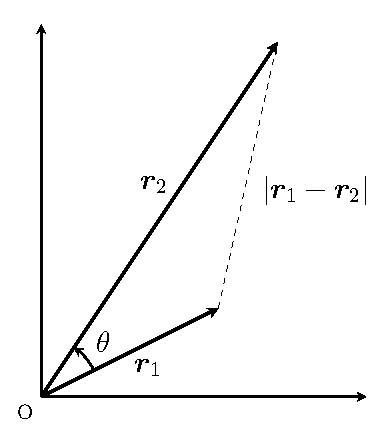
\includegraphics[width=40mm]{../TikZ/multipole/multipole.pdf}
    \label{fig:multipole}
 \end{minipage}
  \end{tabular}
\end{figure}
\end{ibox}
以下では\eqref{eq:Pn-multipole}の証明を行う。
余弦定理を用いて
\begin{equation*}
  \frac{1}{|\bm{r}_1 - \bm{r}_2|}
	= \frac{1}{\sqrt{r_>^2 + r_<^2 - 2r_> r_< \cos\theta}}
	= \frac{1}{r_>} \frac{1}{\sqrt{1 - 2 \cos\theta \cdot \frac{r_<}{r_>} + \( \frac{r_<}{r_>} \)^2}}
\end{equation*}
ここでLegendre多項式の母関数\eqref{eq:Pn-gene}で
$x= \cos\theta, \ t=\frac{r_<}{r_>} $とおいた形が現れているので、
\begin{equation*}
  \frac{1}{|\bm{r}_1 - \bm{r}_2|} = \frac{1}{r_>} \sum_{n=0}^\infty P_n (\cos\theta) \( \frac{r_<}{r_>} \)^n
\end{equation*}
と書き換えられることが示される。

\section{Legendre陪関数}
\subsection{Legendre陪関数}
\label{subsec:associate-legendre}
Legendre陪関数$P_n^m(x)$はRodiguesの公式\eqref{eq:Pnm-Rodrigues}によって定義する
\footnote{この定義にさらに位相因子$(-1)^m$をつけたものを定義として採用する教科書も存在する。
その場合、次節の球面調和関数の定義\eqref{eq:Ylm-def-1}のほうに位相因子$(-1)^m$をつけないことが多い。}
。
定義\eqref{eq:Pnm-Rodrigues}が意味を持つためには次数$m$が$-n\leq m \leq n$なる条件を満たす必要がある。
定義から分かるように$P_n^m(x)$は$m$の値によっては式に$\sqrt{1-x^2}$を含む場合があるので、
一般には多項式にはならず、普通はLegendre陪多項式とは呼ばない(呼ぶ教科書はある)。
特に$m \geq 0$では定義\eqref{eq:Pnm-Rodrigues}は\eqref{eq-Pnm-m>=0}のように
Legendre多項式$P_n(x)$の$m$階導関数を用いて簡潔に表すことができる。
また$m=0$とすると$P_n^m(x)$は$P_n(x)$と一致する。

Legendre陪関数において最も重要な性質は対称性\eqref{eq:Pnm-symmetry}であり、
これは$P_n^{-m} (x)$と$P_n^m(x)$が定数倍を除いて一致することを意味する。
対称性は直交性\eqref{eq:Pnm-chokko}の証明や後述の球面調和関数の理論に絶大な威力を発揮する。

Legendre陪関数はLegendre多項式同様、多数の漸化式を作ることができるが、
ここでは必要最小限の公式だけを載せるにとどめた。

\subsubsection*{公式集}

\paragraph{Rodriguesの公式(定義)}
\begin{equation}\label{eq:Pnm-Rodrigues}
  P_n^m(x) = \frac{1}{2^n \, n!} (1-x^2)^\frac{m}{2} \dx{n+m} (x^2-1)^n \qquad 
  \(
  \begin{array}{c}
    n=0, 1, 2, \dots \\
    -n \leq m \leq n
  \end{array}\small
  \)
\end{equation}

\paragraph{$m\geq0$の場合}
\begin{equation}\label{eq-Pnm-m>=0}
  P_n^m(x) = (1-x^2)^{\frac{m}{2}} \dx{m} P_n(x) \qquad
  \(
  \begin{array}{c}
    n=0, 1, 2, \dots \\
    0 \leq m \leq n
  \end{array}\small
  \)
\end{equation}

\paragraph{$m=0$の場合}
\begin{equation}
  P_n^0 (x) = P_n(x)
\end{equation}

\paragraph{$x=\pm1$での特殊値}
$m \neq 0$のとき
\begin{equation}
  P_n^m(\pm 1) = 0
\end{equation}

\paragraph{偶奇性}
\begin{equation}
  P_n^m(-x) = (-1)^{n+m} P_n^m(x)
\end{equation}

\paragraph{対称性}
\begin{equation}\label{eq:Pnm-symmetry}
  P_n^{-m} (x) = (-1)^m \frac{(n-m)!}{(n+m)!} P_n^m (x)
\end{equation}

\paragraph{昇降演算子}
\begin{alignat}{2}
  &\textbf{上昇演算子}  &\qquad
	& \[ (1-x^2)\dx{} + mx \]P_n^m(x) = \sqrt{1-x^2} P_n^{m+1}(x) \label{eq:Pnm-josho}\\
  &\textbf{下降演算子}  &\qquad
	& \[ (1-x^2)\dx{} - mx \]P_n^m(x) = -(n+m)(n-m+1) \sqrt{1-x^2} P_n^{m-1}(x) \label{eq:Pnm-kako}
\end{alignat}


\paragraph{漸化式($n$固定)}
\begin{equation}\label{eqPnm-req-nfixed}
  \frac{2mx}{\sqrt{1-x^2}} P_n^m(x)
	= P_n^{m+1} (x) + (n+m)(n-m+1) P_n^{m-1}(x)
\end{equation}

\paragraph{漸化式($m$固定)}
\begin{equation}\label{eqPnm-req-mfixed}
  (2n+1)x \, P_n^m(x) = (n+m) P_{n-1}^m (x) + (n-m+1) P_{n+1}^m (x)
\end{equation}


\paragraph{微分方程式}
\begin{equation}
  \[ (1-x^2)\dx{2} -2x \dx{} + \left\{ n(n+1) - \frac{m^2}{1-x^2} \right\} \] P_n^m(x) = 0
\end{equation}

\paragraph{自己随伴形}
\begin{equation}
  \[ \dx{} \left\{ (1-x^2)\dx{}\right\} + \left\{ n(n+1) - \frac{m^2}{1-x^2} \right\} \] P_n^m(x) = 0
\end{equation}


\paragraph{直交性}
\begin{equation}\label{eq:Pnm-chokko}
  \int_{-1}^1 P_n^m(x) P_{n^\prime}^m (x) dx
	= \frac{2}{2n+1} \frac{(n+m)!}{(n-m)!} \delta_{n n^\prime}
\end{equation}


\vspace{-12pt}
\begin{figure}[tb]
\begin{tabular}{cc}
  \hspace{-24pt}
 \begin{minipage}{0.50\hsize}\small
    \begin{table}[H]
      \centering
      \caption{Legendre陪関数 $P_n^m(x) \ (m>0)$}\small
      \begin{tabular}{l}\Hline
        $P_1^1(x) \ = \ \sqrt{1-x^2}$ \\\hdashline
        $P_2^1(x) \ = \ 3x\sqrt{1-x^2}$ \\
        $P_2^2(x) \ = \ 3(1-x^2)$ \\\hdashline
        $P_3^1(x) \ = \ \frac{3}{2} (5x^2-1) \sqrt{1-x^2}$ \\
        $P_3^2(x) \ = \ 15x(1-x^2)$ \\
        $P_3^3(x) \ = \ 15(1-x^2) \sqrt{1-x^2}$ \\\hdashline
        $P_4^1(x) \ = \ \frac{5}{2}(7x^3-3x) \sqrt{1-x^2}$ \\
        $P_4^2(x) \ = \ \frac{15}{2}(7x^2-1) (1-x^2)$ \\
        $P_4^3(x) \ = \ 105x(1-x^2)\sqrt{1-x^2}$\\
        $P_4^4(x) \ = \ 105(1-x^2)^2 $\\\hline
      \end{tabular}
    \end{table}
 \end{minipage}

\hspace{-12pt}
 \begin{minipage}{0.50\hsize}
    \begin{table}[H]
      \centering
      \caption{Legendre陪関数 $P_n^m(x) \ (m<0)$}\small
      \begin{tabular}{l}\Hline
        $P_1^{-1}(x) \ = \ -\frac{1}{2}\sqrt{1-x^2}$ \\\hdashline
        $P_2^{-1}(x) \ = \ -\frac{1}{2}x\sqrt{1-x^2}$ \\
        $P_2^{-2}(x) \ = \ \frac{1}{8}(1-x^2)$ \\\hdashline
        $P_3^{-1}(x) \ = \ -\frac{1}{8} (5x^2-1) \sqrt{1-x^2}$ \\
        $P_3^{-2}(x) \ = \ \frac{1}{8}x(1-x^2)$ \\
        $P_3^{-3}(x) \ = \ -\frac{1}{48}(1-x^2) \sqrt{1-x^2}$ \\\hdashline
        $P_4^{-1}(x) \ = \ -\frac{1}{48}(7x^3-3x) \sqrt{1-x^2}$ \\
        $P_4^{-2}(x) \ = \ \frac{1}{48}(7x^2-1) (1-x^2)$ \\
        $P_4^{-3}(x) \ = \ -\frac{1}{48}x(1-x^2)\sqrt{1-x^2}$\\
        $P_4^{-4}(x) \ = \ \frac{1}{384}(1-x^2)^2 $\\\hline
      \end{tabular}
    \end{table}
  \end{minipage}
\end{tabular}
\end{figure}


% 図
\begin{figure}[tb]
\begin{tabular}{cc}
\hspace{-24pt}
 \begin{minipage}{0.50\hsize}\small
    \begin{figure}[H]
      \centering
      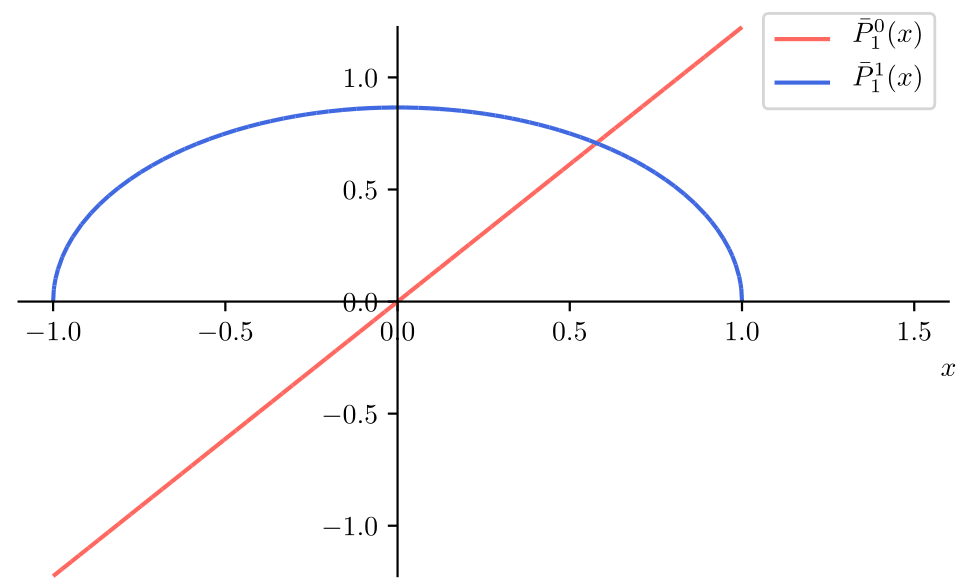
\includegraphics[width=75mm]{../fig/legendre/assoc_legendre1.png}
    \end{figure}
 \end{minipage}

 \begin{minipage}{0.50\hsize}
    \begin{figure}[H]
      \centering
      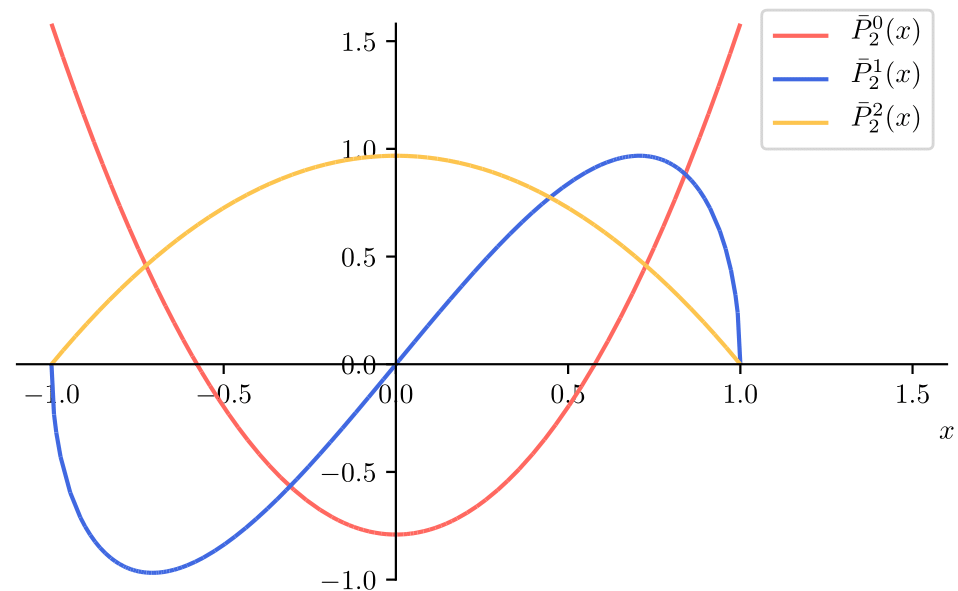
\includegraphics[width=75mm]{../fig/legendre/assoc_legendre2.png}
    \end{figure}
 \end{minipage}
\end{tabular}

\begin{tabular}{cc}
\hspace{-24pt}
 \begin{minipage}{0.50\hsize}
    \begin{figure}[H]
      \centering
      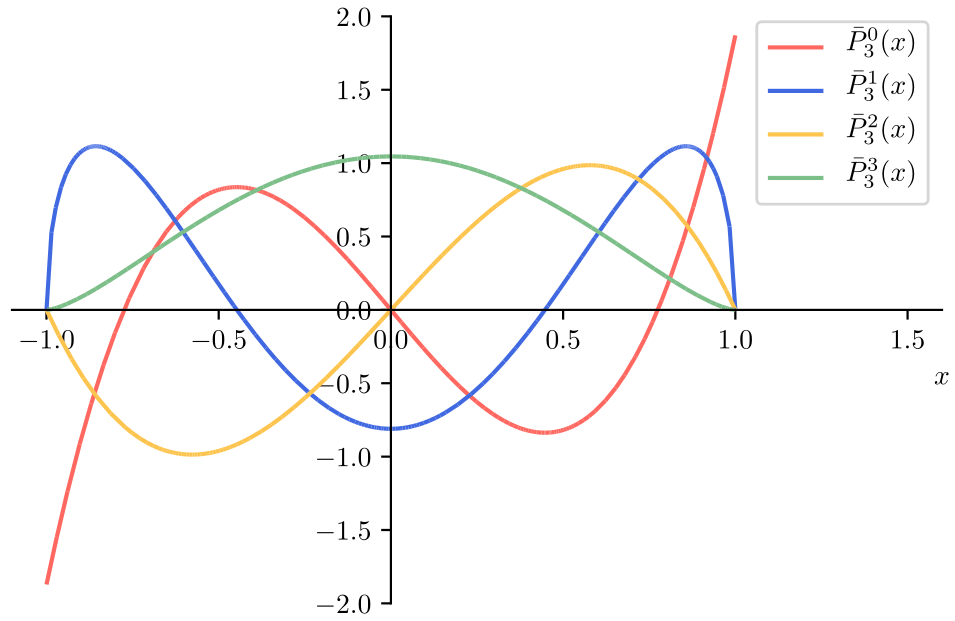
\includegraphics[width=75mm]{../fig/legendre/assoc_legendre3.png}
    \end{figure}
 \end{minipage}

 \begin{minipage}{0.50\hsize}
    \begin{figure}[H]
      \centering
      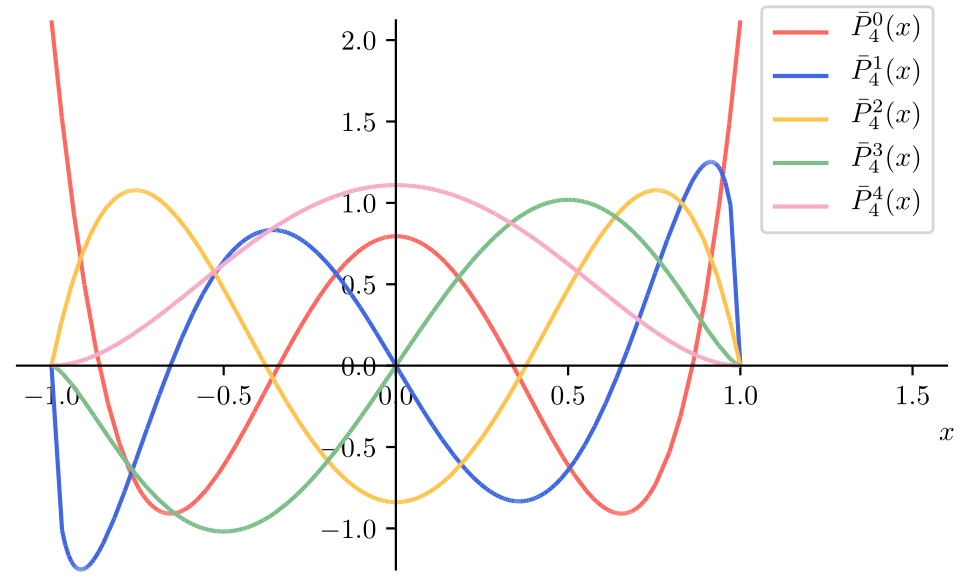
\includegraphics[width=75mm]{../fig/legendre/assoc_legendre4.png}
    \end{figure}
 \end{minipage}
\end{tabular}
\caption{規格化されたLegendre陪関数 
			$\bar{P}_n^m(x) = \sqrt{\frac{2n+1}{2} \frac{(n-m)!}{(n+m)!}} P_n^m(x)$}
\end{figure}


\subsubsection*{証明}
定義\eqref{eq:Pnm-Rodrigues}から$m\geq0$の場合、$m=0$の場合、
$x=\pm1$での特殊値、偶奇性はただちに得られるので、
これらの詳細は省略する。

\paragraph{Rodriguesの公式(定義) $\Longrightarrow$ 対称性}
定義\eqref{eq:Pnm-Rodrigues}に含まれる$n+m$階微分をLeibnizの公式\eqref{eq:Leibniz}によって展開する。
\begin{align}
  &\hspace{-24pt} \dx{n+m} (x^2-1)^n \notag\\
	&= \dx{n+m} (x+1)^n (x-1)^n \notag\\
	&= \sum_{i=0}^{n+m} \binom{n+m}{i}
		\[ \dx{n+m-i} (x+1)^n \] \[ \dx{i} (x-1)^n \] \notag\\
	&= \sum_{i=m}^{n} \binom{n+m}{i}
		\[ \dx{n+m-i} (x+1)^n \] \[ \dx{i} (x-1)^n \] \notag\\
	&= \sum_{i=0}^{n-m} \binom{n+m}{m+i}
		\[ \dx{n-i} (x+1)^n \] \[ \dx{m+i} (x-1)^n \] \notag\\
	&= \sum_{i=0}^{n-m} \frac{(n+m)!}{(m+i)! \, (n-i)!}\cdot
		\frac{n!}{i!} (x+1)^i \cdot \frac{n!}{(n-m-i)!} (x-1)^{n-m-i} \notag\\
	&= (n+m)! \sum_{i=0}^{n-m} \frac{n!}{i!\,(n-i)!} \cdot \frac{n!}{(m+i)!\, (n-m-i)!}
		\cdot (x+1)^i (x-1)^{n-m-i} \notag\\
	&= (n+m)! \sum_{i=0}^{n-m} \binom{n}{i} \binom{n}{m+i} (x+1)^i (x-1)^{n-m-i} \notag
\end{align}
よって
\begin{align}
  P_n^m(x) 
	&= \frac{1}{2^n \, n!} (1-x^2)^\frac{m}{2} \dx{n+m} (x^2-1)^n\notag\\
	&= (n+m)! \cdot \frac{1}{2^n \, n!} (1-x^2)^\frac{m}{2}
		\sum_{i=0}^{n-m} \binom{n}{i} \binom{n}{m+i} (x+1)^i (x-1)^{n-m-i} 
		\label{eq:Pnm-def->symmetry-1}
\end{align}
一方、
\begin{align*}
    &\hspace{-24pt} \dx{n-m} (x^2-1)^n \notag\\
	&= \dx{n-m} (x+1)^n (x-1)^n \notag\\
	&= \sum_{i=0}^{n-m} \binom{n-m}{i}
		\[ \dx{n-m-i} (x+1)^n \] \[ \dx{i} (x-1)^n \] \notag\\
	&= \sum_{i=0}^{n-m} \frac{(n-m)!}{i!\,(n-m-i)!}\cdot
		\frac{n!}{(m+i)!} (x+1)^{m+i} \cdot \frac{n!}{(n-i)!} (x-1)^{n-i} \notag\\
	&= (n-m)! \sum_{i=0}^{n-m} \frac{n!}{i!\, (n-i)!} \cdot \frac{n!}{(m+i)!\, (n-m-i)!}
		\cdot (x+1)^{m+i} (x-1)^{n-i} \notag\\
	&= (n-m)! \sum_{i=0}^{n-m} \binom{n}{i} \binom{n}{m+i} (x+1)^{m+i} (x-1)^{n-i} \notag
\end{align*}
よって
\begin{align}
  P_n^{-m}(x)
	&= \frac{1}{2^n \, n!} (1-x^2)^{-\frac{m}{2}} \dx{n-m} (x^2-1)^n\notag\\
	&= (n-m)!  \cdot \frac{1}{2^n \, n!} (1-x^2)^{-\frac{m}{2}} 
		 \sum_{i=0}^{n-m} \binom{n}{i} \binom{n}{m+i} (x+1)^{m+i} (x-1)^{n-i} \notag\\
	&= (-1)^m  (n-m)! \cdot \frac{1}{2^n \, n!} (1-x^2)^\frac{m}{2}
		\sum_{i=0}^{n-m} \binom{n}{i} \binom{n}{m+i} (x+1)^i (x-1)^{n-m-i} 
		\label{eq:Pnm-def->symmetry-2}
\end{align}
\eqref{eq:Pnm-def->symmetry-1}, \eqref{eq:Pnm-def->symmetry-2}を比較して次を得る。
\begin{equation*}
  P_n^{-m} (x) = (-1)^m \frac{(n-m)!}{(n+m)!} P_n^m (x)
\end{equation*}\qed


\paragraph{定義 $\Longrightarrow$ 上昇演算子}
$\dx{} \[ (1-x^2)^{-\frac{m}{2}} P_n^m(x) \]$を2通りに変形する。
まず定義\eqref{eq:Pnm-Rodrigues}を用いて
\begin{align}
  \dx{} \[ (1-x^2)^{-\frac{m}{2}} P_n^m(x) \]
	&= \dx{} \[ (1-x^2)^{-\frac{m}{2}} \cdot \frac{1}{2^n \, n!}
		 (1-x^2)^\frac{m}{2} \dx{n+m} (x^2-1)^n \] \notag\\
	&= \frac{1}{2^n \, n!} \dx{n+m+1} (x^2-1)^n \notag\\
	&= (1-x^2)^{-\frac{m+1}{2}} \[ \frac{1}{2^n \, n!} (1-x^2)^{\frac{m+1}{2}}
		\dx{n+m+1} (x^2-1)^n \] \notag\\
	&=  (1-x^2)^{-\frac{m+1}{2}} P_n^{m+1} (x)
		\label{eq:Pnm-def->josho-1}
\end{align}
一方、1階微分を実行すると
\begin{align}
  \dx{} \[ (1-x^2)^{-\frac{m}{2}} P_n^m(x) \] 
	&= (1-x^2)^{-\frac{m}{2}} \dx{} P_n^m (x) + mx (1-x^2)^{-\frac{m}{2}-1} P_n^m(x) \notag\\
	&= (1-x^2)^{-\frac{m}{2}-1} \[  (1-x^2)\dx{} + mx  \] P_n^m (x) 
		\label{eq:Pnm-def->josho-2}
\end{align}
\eqref{eq:Pnm-def->josho-1}, \eqref{eq:Pnm-def->josho-2}より
\begin{equation*}
  (1-x^2)^{-\frac{m}{2}-1} \[  (1-x^2)\dx{} + mx  \] P_n^m (x) 
	= (1-x^2)^{-\frac{m+1}{2}} P_n^{m+1} (x)
\end{equation*}
両辺を$(1-x^2)^{\frac{m}{2}+1}$倍して次を得る。
\begin{equation*}
  \[ (1-x^2)\dx{} + mx \]P_n^m(x) = \sqrt{1-x^2} P_n^{m+1}(x) 
\end{equation*}\qed

\paragraph{上昇演算子, 対称性 $\Longrightarrow$ 下降演算子}
上昇演算子\eqref{eq:Pnm-josho}において$m$を$-m$に置きかえると
\begin{equation}\label{eq:Pnm-josho->kako}
  \[ (1-x^2)\dx{} - mx \]P_n^{-m}(x) = \sqrt{1-x^2} P_n^{-m+1}(x)
\end{equation}
ここで対称性\eqref{eq:Pnm-symmetry}から
\begin{align*}
  &P_n^{-m} (x) = (-1)^m \frac{(n-m)!}{(n+m)!} P_n^m (x) \notag\\
  &P_n^{-m+1} (x) = (-1)^{m-1} \frac{(n-m+1)!}{(n+m-1)!} P_n^{m-1} (x)
\end{align*}
であるので、これらを\eqref{eq:Pnm-josho->kako}に代入して整理すると次が得られる。
\begin{equation*}
  \[ (1-x^2)\dx{} - mx \]P_n^m(x) = -(n+m)(n-m+1) \sqrt{1-x^2} P_n^{m-1}(x)
\end{equation*}\qed


\paragraph{昇降演算子 $\Longrightarrow$ 漸化式($n$固定)}
$\eqref{eq:Pnm-josho} - \eqref{eq:Pnm-kako}$により、昇降演算子の微分を含む項を消去して
整理すると、$n$が固定された漸化式\eqref{eqPnm-req-nfixed}が得られる。\qed

\vspace{10pt}
\paragraph{定義, $P_n (x)$の漸化式, 対称性 $\Longrightarrow$ 漸化式($m$固定)}
$m$が固定された漸化式は、Legendre多項式についての漸化式を用いて示す。

\vspace{6pt}
\underline{$m\geq 0$のとき}
\begin{equation*}
   (2n+1)x \, P_n^m(x) 
	= (2n+1) x  (1-x^2)^{\frac{m}{2}} \dx{m} P_n(x)
\end{equation*}
ここでLeibnizの公式\eqref{eq:Leibniz}から
\begin{equation*}
  \dx{m} \left\{ xP_n(x) \right\}
	= x \dx{m} P_n(x) + m \dx{m-1} P_n(x) \quad \iff \quad
	x \dx{m} P_n(x) = \dx{m} \left\{ xP_n(x) \right\} - m \dx{m-1} P_n(x) 
\end{equation*}
であるから、
\begin{align}
  (2n+1)x \, P_n^m(x) 
	&= (2n+1) (1-x^2)^{\frac{m}{2}} \[ \dx{m} \left\{ xP_n(x) \right\} - m \dx{m-1} P_n(x) \] \notag\\
	&\, \downarrow \quad 三項間漸化式 \eqref{eq:Pn-req-3ko}, \eqref{eq:Pn-diff-req-3ko-II} \notag\\
	&= (1-x^2)^{\frac{m}{2}} \[ \dx{m} \left\{ n P_{n-1}(x) + (n+1) P_{n+1} (x) \right\} 
		-m \dx{m-1} \left\{ -P_{n-1}^\prime (x) + P_{n+1}^\prime (x)  \right\} \] \notag\\
	&= (1-x^2)^{\frac{m}{2}} \[ (n+m) \dx{m} P_{n-1}(x)
			+ (n-m+1) \dx{m} P_{n+1}(x) \] \notag\\
	&= (n+m) P_{n-1}^m (x) + (n-m+1) P_{n+1}^m (x) \label{eq:Pnm-def->req-mfixed-En}
\end{align}

\underline{$m\leq 0$のとき} \ 対称性\eqref{eq:Pnm-symmetry}を用いて
\eqref{eq:Pnm-def->req-mfixed-En}を書き換えると、
\begin{align*}
  &\hspace{-24pt} (2n+1)x \, \cdot (-1)^{m} \frac{(n+m)!}{(n-m)!}  P_n^{-m}(x) \notag\\
	&=  (n+m)\cdot (-1)^m \frac{(n+m-1)!}{(n-m-1)!} P_{n-1}^{-m} (x) 
		+ (n-m+1) \cdot (-1)^{-m} \frac{(n+m+1)!}{(n-m+1)!} P_{n+1}^{-m} (x) \notag
\end{align*}
両辺を$(-1)^m \frac{(n-m)!}{(n+m)!}$倍して整理すると
\begin{equation*}
  (2n+1)x \, P_n^{-m}(x) 
	= (n-m) P_{n-1}^{-m} (x) + (n+m+1) P_{n+1}^{-m} (x)
\end{equation*}
この式は\eqref{eq:Pnm-def->req-mfixed-En}で$m$を$-m$に置きかえた形となっており、
\eqref{eq:Pnm-def->req-mfixed-En}が$m \leq 0$に対しても成立することを表す。

\vspace{6pt}
以上をまとめると、$-n \leq m \leq n$を満たすすべての$m$に対して次が成り立つことが示された。
\begin{equation*}
  (2n+1)x \, P_n^m(x) = (n+m) P_{n-1}^m (x) + (n-m+1) P_{n+1}^m (x)
\end{equation*}\qed


\paragraph{昇降演算子 $\Longrightarrow$ 微分方程式}
昇降演算子\eqref{eq:Pnm-josho}, \eqref{eq:Pnm-kako}を次のように書き直しておく。
\begin{alignat}{2}
  &\textbf{上昇演算子}  &\qquad
	&\[ \sqrt{1-x^2} \dx{} + \frac{mx}{\sqrt{1-x^2}} \]P_n^m(x) =  P_n^{m+1}(x) 
		\label{eq:Pnm-shoko->diff-josho}\\
  &\textbf{下降演算子}  &\qquad
	&\[ \sqrt{1-x^2} \dx{} - \frac{mx}{\sqrt{1-x^2}} \]P_n^m(x) = -(n+m)(n-m+1) P_n^{m-1}(x) 
		\label{eq:Pnm-shoko->diff-kako}
\end{alignat}
上昇演算子\eqref{eq:Pnm-shoko->diff-josho}の両辺に
左から$\[ \sqrt{1-x^2} \dx{} - \frac{(m+1)x}{\sqrt{1-x^2}} \]$を作用させると、左辺は
\begin{align*}
  &\hspace{-24pt} \[ \sqrt{1-x^2} \dx{} - \frac{(m+1)x}{\sqrt{1-x^2}} \]
		\[ \sqrt{1-x^2} \dx{} + \frac{mx}{\sqrt{1-x^2}} \] P_n^m(x) \notag\\
	&= \[ \sqrt{1-x^2} \dx{} \left\{ \sqrt{1-x^2} \dx{} + \frac{mx}{\sqrt{1-x^2}} \right\}
		- \frac{(m+1)x}{\sqrt{1-x^2}} \left\{ \sqrt{1-x^2} \dx{} + \frac{mx}{\sqrt{1-x^2}} \right\} \] P_n^m(x)
		\notag\\
	&= \[ \sqrt{1-x^2} \left\{ \frac{-x}{\sqrt{1-x^2}} \dx{} + \sqrt{1-x^2} \dx{2}
			+ \frac{m\sqrt{1-x^2} - mx\cdot \frac{-x}{\sqrt{1-x^2}}}{1-x^2} 
			+ \frac{mx}{\sqrt{1-x^2}} \dx{} \right\} \right. \notag\\ 
		&\hspace{48pt} \left. - \left\{ (m+1)x \dx{} - \frac{m(m+1)}{1-x^2}x^2 \right\} \] P_n^m(x)
		\notag\\
	&= \[ (1-x^2)\dx{2} - 2x \dx{} + \frac{m-m(m+1)x^2}{1-x^2} \] P_n^m(x)
\end{align*}
一方、右辺は下降演算子\eqref{eq:Pnm-shoko->diff-kako}を用いて
\begin{align*}
  \[ \sqrt{1-x^2} \dx{} - \frac{(m+1)x}{\sqrt{1-x^2}} \] P_n^{m+1}(x) 
	&= -(n+m+1)(n-m) P_n^m(x) \notag\\
	&= \left\{ -n(n+1) + m(m+1) \right\} P_n^m(x)
\end{align*}
となるので、
\begin{gather*}
  \[ (1-x^2)\dx{2} - 2x \dx{} + \frac{m-m(m+1)x^2}{1-x^2} \] P_n^m(x)
	= \left\{ -n(n+1) + m(m+1) \right\} P_n^m(x) \notag\\ \therefore
  \[ (1-x^2)\dx{2} -2x \dx{} + \left\{ n(n+1) - \frac{m^2}{1-x^2} \right\} \] P_n^m(x) = 0
\end{gather*}
また、この方程式は次のようにも変形できる。
\begin{equation*}
  \[ \dx{} \left\{ (1-x^2)\dx{}\right\} + \left\{ n(n+1) - \frac{m^2}{1-x^2} \right\} \] P_n^m(x) = 0
\end{equation*}\qed

\paragraph{$P_n(x)$の直交性, 対称性 $\Longrightarrow$ 直交性}
対称性\eqref{eq:Pnm-symmetry}を用いて
\eqref{eq:Pnm-chokko}の左辺を書き換えると
\begin{equation}\label{eq-Pnm-sym->choko}
   \int_{-1}^1 P_n^m(x) P_{n^\prime}^m (x) dx
	= (-1)^m \frac{(n+m)!}{(n-m)!} \int_{-1}^1 P_n^{-m}(x) P_{n^\prime}^m (x) dx
\end{equation}
ここで
\begin{equation*}
  I_m = \int_{-1}^1 P_n^{-m}(x) P_{n^\prime}^m (x) dx
\end{equation*}
とおくと、1回の部分積分により次のような関係が成り立つことが分かる
\footnote{難しい計算はないので、各自で確認してみて欲しい。}
。
\begin{equation*}
  I_m = - I_{m-1}
\end{equation*}
これを繰り返し用いると
\begin{equation*}
  I_m = (-1)^m I_0
	= (-1)^m \int_{-1}^1 P_n (x) P_{n^\prime} (x) dx
	\overset{\eqref{eq:Pn-choko}}{=} (-1)^m \frac{2}{2n+1} \delta_{n n^\prime}
\end{equation*}
となるので、\eqref{eq-Pnm-sym->choko}に代入して次が得られる。
\begin{equation*}
  \int_{-1}^1 P_n^m(x) P_{n^\prime}^m (x) dx
	= \frac{2}{2n+1} \frac{(n+m)!}{(n-m)!} \delta_{n n^\prime}
\end{equation*}\qed


\subsection{$P_n^m (\cos \theta)$についての公式}

%表
\begin{figure}[tb]
\begin{tabular}{cc}
  \hspace{-24pt}
 \begin{minipage}{0.50\hsize}\small
    \begin{table}[H]
      \centering
      \caption{Legendre多項式 $P_n(\cos\theta)$}\small
      \begin{tabular}{l}\Hline
        $P_0(\cos\theta) \ = \ 1$\\
        $P_1(\cos\theta) \ = \ \cos\theta$\\
        $P_2(\cos\theta) \ = \ \frac{1}{2} (3\cos^2\theta - 1)$ \\
        $P_3(\cos\theta) \ = \ \frac{1}{2} (5\cos^3\theta - 3\cos\theta)$ \\
        $P_4(\cos\theta) \ = \ \frac{1}{8} (35\cos^4\theta - 30 \cos^2\theta + 3)$ \\
        $P_5(\cos\theta) \ = \ \frac{1}{8} (63\cos^5\theta - 70 \cos^3\theta + 15\cos\theta)$ \\
        $P_6(\cos\theta) \ = \ \frac{1}{16} (231\cos^6\theta 
		- 315\cos^4\theta + 105\cos^2\theta - 5)$ \\\hline
      \end{tabular}
    \end{table}
 \end{minipage}

    \hspace{12pt}
   \begin{minipage}{0.50\hsize}
     \begin{figure}[H]
       \centering
       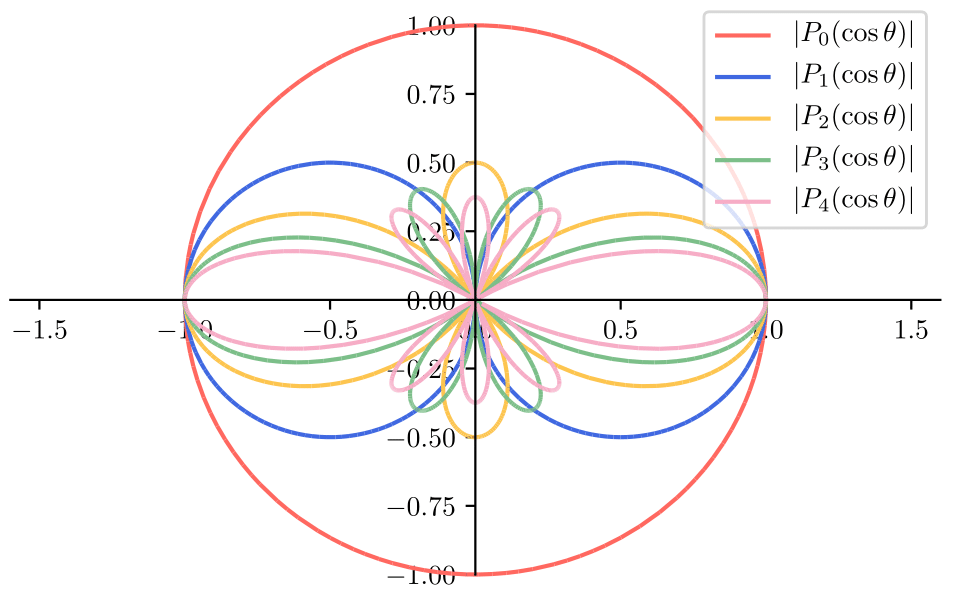
\includegraphics[width=75mm]{../fig/legendre/legendre_cos.png}
     \end{figure} \vspace{-6pt}\small
     \caption{Legendre多項式 $P_n(\cos\theta)$\newline
		偏角$\theta$に対する$|P_n(\cos\theta)|$の値を原点からの距離として表現している}\small
  \end{minipage}
\end{tabular}
\end{figure}



実際の計算では、Legendre陪関数は$P_n^m(\cos\theta)$の形で現れることが多い。
そこで、前\ref{subsec:associate-legendre}節で挙げた公式を$P_n^m(\cos\theta)$についての公式に
書き換えたものの一部をここで列挙しておこう。
確認するには$x=\cos\theta$として、
\begin{align*}
  &\frac{d}{dx} = \frac{d}{d(\cos\theta)} = \frac{d\theta}{d(\cos\theta)} \frac{d}{d\theta}
	= \frac{1}{d(\cos\theta)/d\theta} \frac{d}{d\theta}
	= -\frac{1}{\sin\theta} \frac{d}{d\theta} \notag\\
  &\frac{d^2}{dx^2} 
	= \( -\frac{1}{\sin\theta} \frac{d}{d\theta} \) \( -\frac{1}{\sin\theta} \frac{d}{d\theta} \)
	= \frac{1}{\sin\theta} \( \frac{1}{\sin\theta} \frac{d^2}{d\theta^2} 
		- \frac{\cos\theta}{\sin^2\theta} \frac{d}{d\theta}  \)
	= \frac{1}{\sin^2\theta} \frac{d^2}{d\theta^2} - \frac{\cos\theta}{\sin^3\theta} \frac{d}{d\theta}
\end{align*}
などに注意して\ref{subsec:associate-legendre}節の公式集を丁寧に書き直すだけである。
最後の直交性の被積分関数に$\sin\theta$が現れることにも注意しよう。
難しい部分はないので、導出過程の詳細は省略する。

\subsubsection*{公式集}

\paragraph{$m\geq 0$の場合}
\begin{equation}
  P_n^m (\cos\theta)
	= \sin^m\theta \frac{d^m}{d(\cos\theta)^m} P_n(\cos\theta)
\end{equation}


\paragraph{$m=0$の場合}
\begin{equation}
  P_n^0 (\cos\theta) = P_n (\cos \theta)
\end{equation}

\paragraph{偶奇性}
\begin{equation}\label{eq:Pnm-cos-parity}
  P_n^m(-\cos\theta) = (-1)^{m+n} P_n^m(\cos\theta)
\end{equation}


\paragraph{対称性}
\begin{equation}\label{eq:Pnm-cos-sym}
  P_n^{-m} (\cos\theta) = (-1)^m \frac{(n-m)!}{(n+m)!} P_n^m (\cos\theta)
\end{equation}

\paragraph{昇降演算子}
\begin{alignat}{2}
  &\textbf{上昇演算子}  &\qquad
	& \( \frac{d}{d\theta} - m \cot\theta \)P_m^n (\cos\theta)
		= -P_n^{m+1} (\cos\theta) \label{eq:Pnm-cos-josho}\\
  &\textbf{下降演算子}  &\qquad
	& \( \frac{d}{d\theta} + m \cot\theta \)P_m^n (\cos\theta)
		= (n+m)(n-m+1) P_n^{m-1} (\cos\theta) \label{eq:Pnm-cos-kako}
\end{alignat}

\paragraph{微分方程式}
\begin{equation}\label{eq:Pnm-cos-diff-eq}
  \[ \frac{d^2}{d\theta^2} + \cot\theta \frac{d}{d\theta} 
	+ \left\{ n(n+1) - \frac{m^2}{\sin^2\theta} \right\} \] P_n^m(\cos\theta) = 0
\end{equation}


\paragraph{自己随伴形}
\begin{equation}\label{eq:Pnm-cos-self}
  \[ \frac{1}{\sin\theta} \frac{d}{d\theta} \( \sin\theta \frac{d}{d\theta} \)
	+ \left\{ n(n+1) - \frac{m^2}{\sin^2\theta} \right\} \] P_n^m(\cos\theta) = 0
\end{equation}


\paragraph{直交性}
\begin{equation}\label{eq:Pnm-cos-chokko}
  \int_0^\pi P_n^m (\cos\theta) P_{n^\prime}^m (\cos\theta) \sin\theta \, d\theta
	 = \frac{2}{2n+1} \frac{(n+m)!}{(n-m)!} \delta_{n n^\prime}
\end{equation}



% 図
\begin{figure}[tb]
\begin{tabular}{c}
\hspace{-24pt}
 \begin{minipage}{0.50\hsize}\small
    \begin{figure}[H]
      \centering
      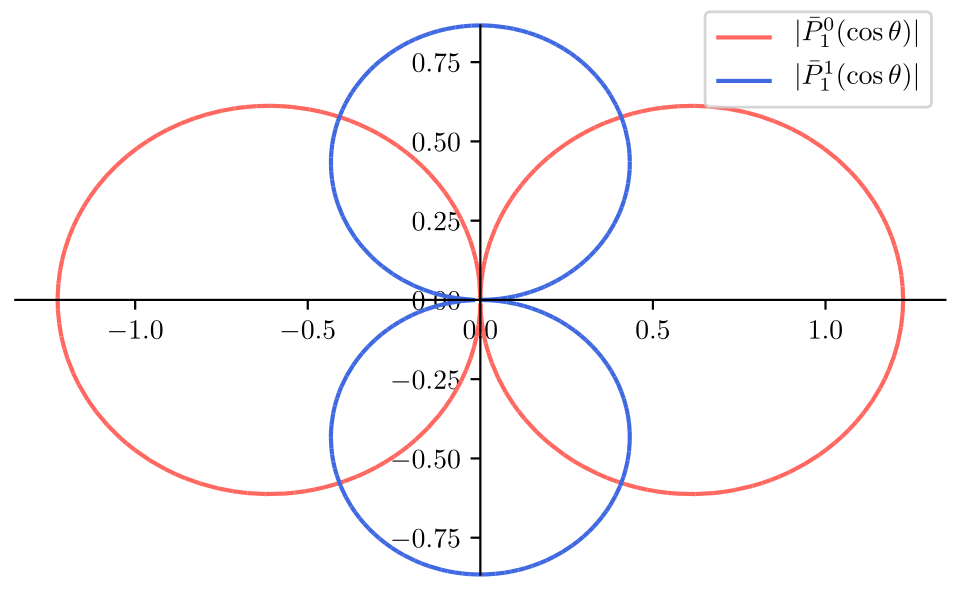
\includegraphics[width=75mm]{../fig/legendre/assoc_legendre_cos1.png}
    \end{figure}
 \end{minipage}

 \begin{minipage}{0.50\hsize}
    \begin{figure}[H]
      \centering
      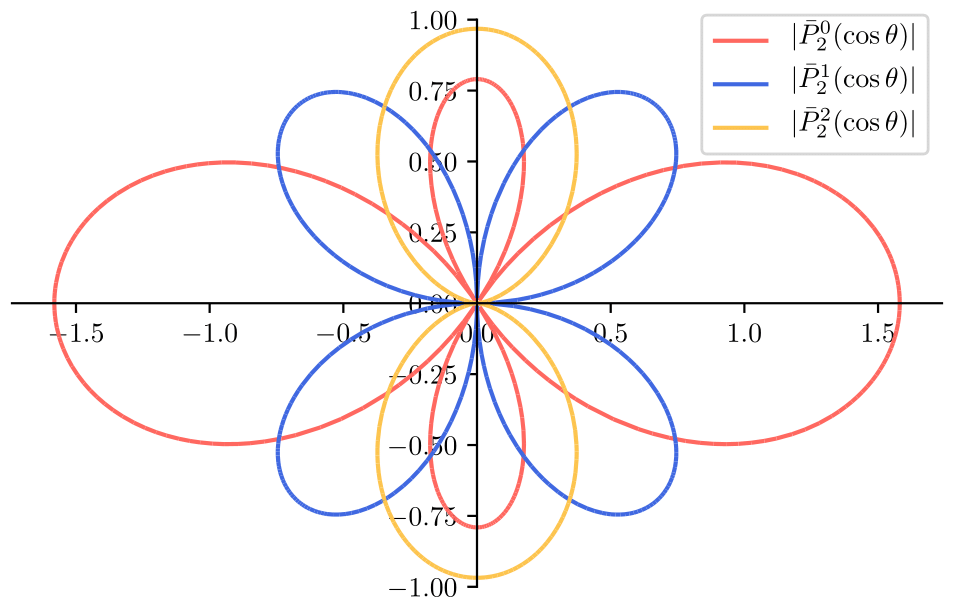
\includegraphics[width=75mm]{../fig/legendre/assoc_legendre_cos2.png}
    \end{figure}
 \end{minipage}
\end{tabular}

\begin{tabular}{cc}
\hspace{-24pt}
 \begin{minipage}{0.50\hsize}
    \begin{figure}[H]
      \centering
      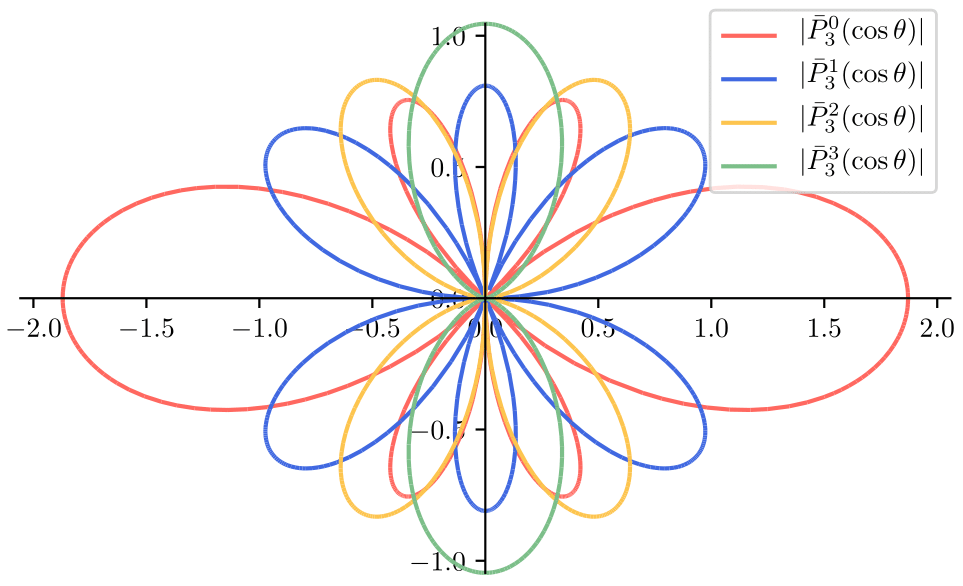
\includegraphics[width=75mm]{../fig/legendre/assoc_legendre_cos3.png}
    \end{figure}
 \end{minipage}

 \begin{minipage}{0.50\hsize}
    \begin{figure}[H]
      \centering
      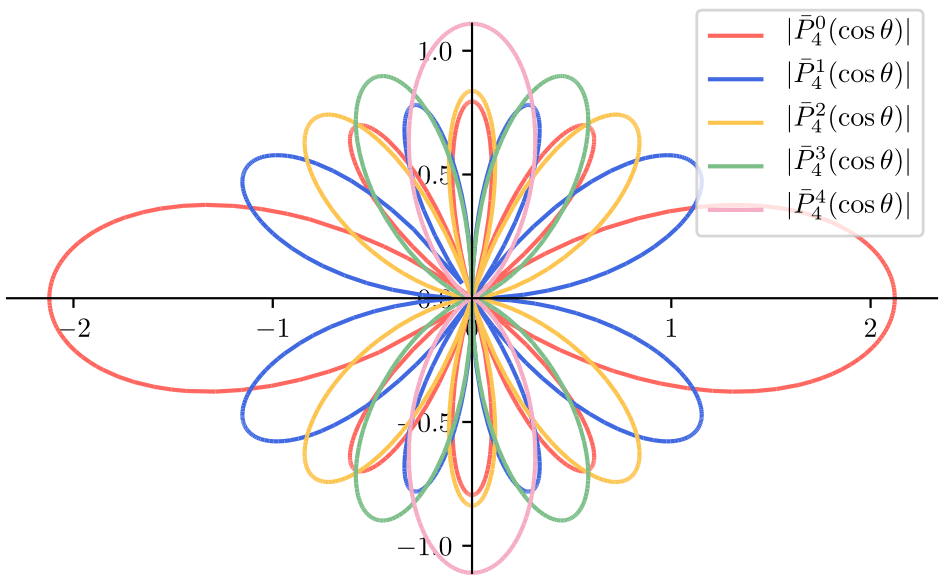
\includegraphics[width=75mm]{../fig/legendre/assoc_legendre_cos4.png}
    \end{figure}
 \end{minipage}
\end{tabular}
\caption{\hspace{24pt}規格化されたLegendre陪関数 
			$\bar{P}_n^m(\cos\theta) = \sqrt{\frac{2n+1}{2} \frac{(n-m)!}{(n+m)!}} P_n^m(\cos\theta)$
		\newline \hspace{52pt}
		偏角$\theta$に対する$|\bar{P}_n^m(\cos\theta)|$の値を原点からの距離として表現している}
\end{figure}




\begin{table}[tb]
  \centering
      \caption{Legendre陪関数 $P_n^m(\cos\theta) \ (m\geq 0)$}\small
      \begin{tabular}{l}\Hline
        $P_1^{1}(\cos\theta) \ = \ \sin\theta$ \\\hdashline
        $P_2^{1}(\cos\theta) \ = \ 3\cos\theta\sin\theta$ \\
        $P_2^{2}(\cos\theta) \ = \ 3\sin^2\theta$ \\\hdashline
        $P_3^{1}(\cos\theta) \ = \ \frac{3}{2} (5\cos^2\theta-1)\sin\theta$ \\
        $P_3^{2}(\cos\theta) \ = \ 15\cos\theta\sin^2\theta$ \\
        $P_3^{3}(\cos\theta) \ = \ 15\sin^3\theta$ \\\hdashline
        $P_4^{1}(\cos\theta) \ = \ \frac{5}{2}(7\cos^3\theta - 3\cos\theta)\sin\theta$ \\
        $P_4^{2}(\cos\theta) \ = \ \frac{15}{2}(7\cos^2\theta-1)\sin^2\theta$ \\
        $P_4^{3}(\cos\theta) \ = \ 105\cos\theta\sin^3\theta$\\
        $P_4^{4}(\cos\theta) \ = \ 105\sin^4\theta$\\\hline
      \end{tabular}
\end{table}


\section{球面調和関数}

\subsection{球面調和関数}
Laplace方程式$\Delta \psi = 0$を球座標系$(r, \theta, \varphi)$で
$\psi = R(r) \Theta(\theta) \Phi (\varphi)$と変数分離してしかるべき条件
\footnote{
$\varphi$について一価関数であること、および$\theta=0, \pi$において有限であること。

}
のもと解くと、
方位角$\varphi$について規格化された$\Phi (\varphi)$と、
天頂角$\theta$について規格化された$\Theta(\theta)$はそれぞれ次のように求められる( 問題[2-2] )。
\begin{alignat}{2}
  \Phi (\varphi) &= \frac{1}{\sqrt{2\pi}} e^{im\varphi} && (m = 0, \pm1, \pm2, \dots) \\
  \Theta(\theta) &= \sqrt{\frac{2l+1}{2} \frac{(l-m)!}{(l+m)!}} \ P_l^m (\cos\theta) &\qquad
	&(-l \leq m \leq l)
\end{alignat}
したがってLaplace方程式の解の球面上で規格化された角度依存性は
\begin{equation*}
  \Theta(\theta) \Phi (\varphi)
	= \sqrt{\frac{2l+1}{4\pi} \frac{(l-m)!}{(l+m)!}} \ P_l^m(\cos\theta) \, e^{im\varphi}
\end{equation*}
と書けることになる。
実はLaplace方程式のみならず、Helmholtz方程式$(\Delta + k^2) \psi = 0$や
波動方程式$(\Delta - \frac{1}{c^2} \frac{\6^2}{\6 t^2}) \psi = 0$, 
中心力場のSchr\"{o}dinger方程式などでもまったく同じ結果が得られる。
そこでこの規格化された角度依存性に位相因子$(-1)^m$を付したものは
しばしば\textbf{球面調和関数}とよばれ、$Y_{lm}(\theta, \varphi)$で表される
\footnote{
位相因子$(-1)^m$を付けない教科書もあるが、その場合Legendre陪関数の定義\eqref{eq:Pnm-Rodrigues}にこの因子をつけられることが多い。
}
。
位相因子$(-1)^m$は必要ないように感じられるが、
このように定義しておくと量子力学の角運動量の理論などにおいて有用になることが多い。
教科書によっては$Y_{lm}(\theta, \varphi)$の定義が\eqref{eq:Ylm-def-2}のように書かれることがあるが、
これは\eqref{eq:Ylm-def-1}と意味することは同じである
\footnote{
\eqref{eq:Ylm-def-2}についている$(-1)^{\frac{m+|m|}{2}}$が次のような性質を持つことは重要である。
\begin{equation}
  (-1)^{\frac{m+|m|}{2}} = \left\{
  \begin{alignedat}{2}
    &(-1)^m 	& \qquad &(m\geq 0) \\
    &1 		& 		& (m \leq 0)
  \end{alignedat}
  \right.
\end{equation}
すなわち、$m \geq 0$のときは$m$の変化により正負の入れ替わりが起こるが、
$m\leq0$のときは常に正になるということである。
教科書によってはこの意味を持つ定数として$\epsilon_m$と定義するものも多い。
}
。
基本的に$Y_{lm}(\theta, \varphi)$についての公式は、
定義\eqref{eq:Ylm-def-1}と$P_n^m(\cos\theta)$についての公式を用いてすぐに導くことができる。

\subsubsection*{公式集}

\paragraph{定義}
\begin{align}
  Y_{lm} (\theta, \varphi)
	&= (-1)^m \sqrt{\frac{2l+1}{4\pi} \frac{(l-m)!}{(l+m)!}} 
		\ P_l^m(\cos\theta) \, e^{im\varphi}
  \qquad \(
  \begin{array}{c}
    l=0, 1, 2, \dots \\
    -l \leq m \leq l
  \end{array}
  \) \label{eq:Ylm-def-1} \\
	&= (-1)^{\frac{m+|m|}{2}} \sqrt{\frac{2l+1}{4\pi} \frac{(l-|m|)!}{(l+|m|)!}} 
	\ P_l^{|m|}(\cos\theta) \, e^{im\varphi} \label{eq:Ylm-def-2}
\end{align}

\paragraph{偶奇性}
\begin{equation}
  Y_{lm}(\pi-\theta, \varphi+\pi) = (-1)^l \ Y_{lm} (\theta, \varphi)
\end{equation}

\paragraph{対称性}
\begin{equation}
  Y_{l, -m} (\theta, \varphi) = (-1)^m \ Y_{lm}(\theta, \varphi)^*
\end{equation}


\paragraph{昇降演算子}
\begin{alignat}{2}
  &\textbf{上昇演算子}& 
	e^{i\varphi} \( \frac{\6}{\6\theta} + i \cot\theta\frac{\6}{\6\varphi} \) Y_{lm} (\theta, \varphi)
		&= \sqrt{(l-m)(l+m+1)} \ Y_{l, m+1} (\theta, \varphi) \label{eq:Ylm-josho}\\
  &\textbf{下降演算子} & \qquad 
	e^{-i\varphi} \( -\frac{\6}{\6\theta} + i \cot\theta\frac{\6}{\6\varphi} \) Y_{lm} (\theta, \varphi)
		&= \sqrt{(l+m)(l-m+1)} \ Y_{l, m-1} (\theta, \varphi) \label{eq:Ylm-kako}
\end{alignat}

\paragraph{微分方程式}
\begin{align}
  &- \[ \frac{1}{\sin\theta} \frac{\6}{\6\theta} \( \sin\theta \frac{\6}{\6\theta} \)
	+ \frac{1}{\sin^2\theta} \frac{\6^2}{\6 \varphi^2} \] Y_{lm} (\theta, \varphi) 
		= l(l+1) \ Y_{lm} (\theta, \varphi) \label{eq:Ylm-diff-eq-1} \\
  &-i \frac{\6}{\6 \varphi} Y_{lm} (\theta, \varphi) = m \, Y_{lm} (\theta, \varphi) 
		\label{eq:Ylm-diff-eq-2}
\end{align}

\paragraph{直交性}
\begin{equation}
  \iint Y_{lm} (\theta, \varphi)^* \, Y_{l^\prime m^\prime} (\theta, \varphi) \, d\Omega
	= \delta_{l l^\prime} \delta_{m m^\prime} 
\end{equation}

% 表
\begin{table}[tb]
  \centering
      \caption{球面調和関数 $Y_{lm} (\theta, \varphi) $}\small
      \begin{tabular}{lcl}\Hline
        $Y_{00}(\theta, \varphi)$ 		& = & $\sqrt{\dfrac{1}{4\pi}}$ \\\hdashline
        $Y_{10}(\theta, \varphi)$ 		& = & $\sqrt{\dfrac{3}{4\pi}} \cos\theta$ \\
        $Y_{1, \pm1}(\theta, \varphi)$ 	& = 
		& $\mp \sqrt{\dfrac{3}{8\pi}} \sin\theta \, e^{\pm i\varphi}$ \\\hdashline
        $Y_{20}(\theta, \varphi)$ 		& = 
		& $\sqrt{\dfrac{5}{16\pi}} (3\cos^2\theta-1)$ \\
        $Y_{2, \pm1}(\theta, \varphi)$ 	& = 
		& $\mp\sqrt{\dfrac{15}{8\pi}}\cos\theta\sin\theta \, e^{\pm i \varphi}$ \\
        $Y_{2, \pm2}(\theta, \varphi)$ 	& = 
		& $\sqrt{\dfrac{15}{32\pi}}\sin^2\theta \, e^{\pm 2i\varphi}$ \\\hdashline
        $Y_{30}(\theta, \varphi)$ 		& = 
		& $\sqrt{\dfrac{7}{16\pi}}(5\cos^3\theta - 3\cos\theta) $ \\
        $Y_{3, \pm1}(\theta, \varphi)$ 	& = 
		& $\mp \sqrt{\dfrac{21}{64\pi}} (5\cos^2\theta-1) \sin\theta \, e^{\pm i\varphi}$ \\
        $Y_{3, \pm2}(\theta, \varphi)$ 	& = 
		& $\sqrt{\dfrac{105}{32\pi}} \cos\theta\sin^2\theta \, e^{\pm 2 i\varphi}$\\
        $Y_{3, \pm3}(\theta, \varphi)$ 	& = 
		& $\mp\sqrt{\dfrac{35}{64\pi}}\sin^3\theta \, e^{\pm 3i\varphi}$\\\hline
      \end{tabular}
      \label{tab:Ylm}
\end{table}

\begin{figure}[tbp]
  \centering
  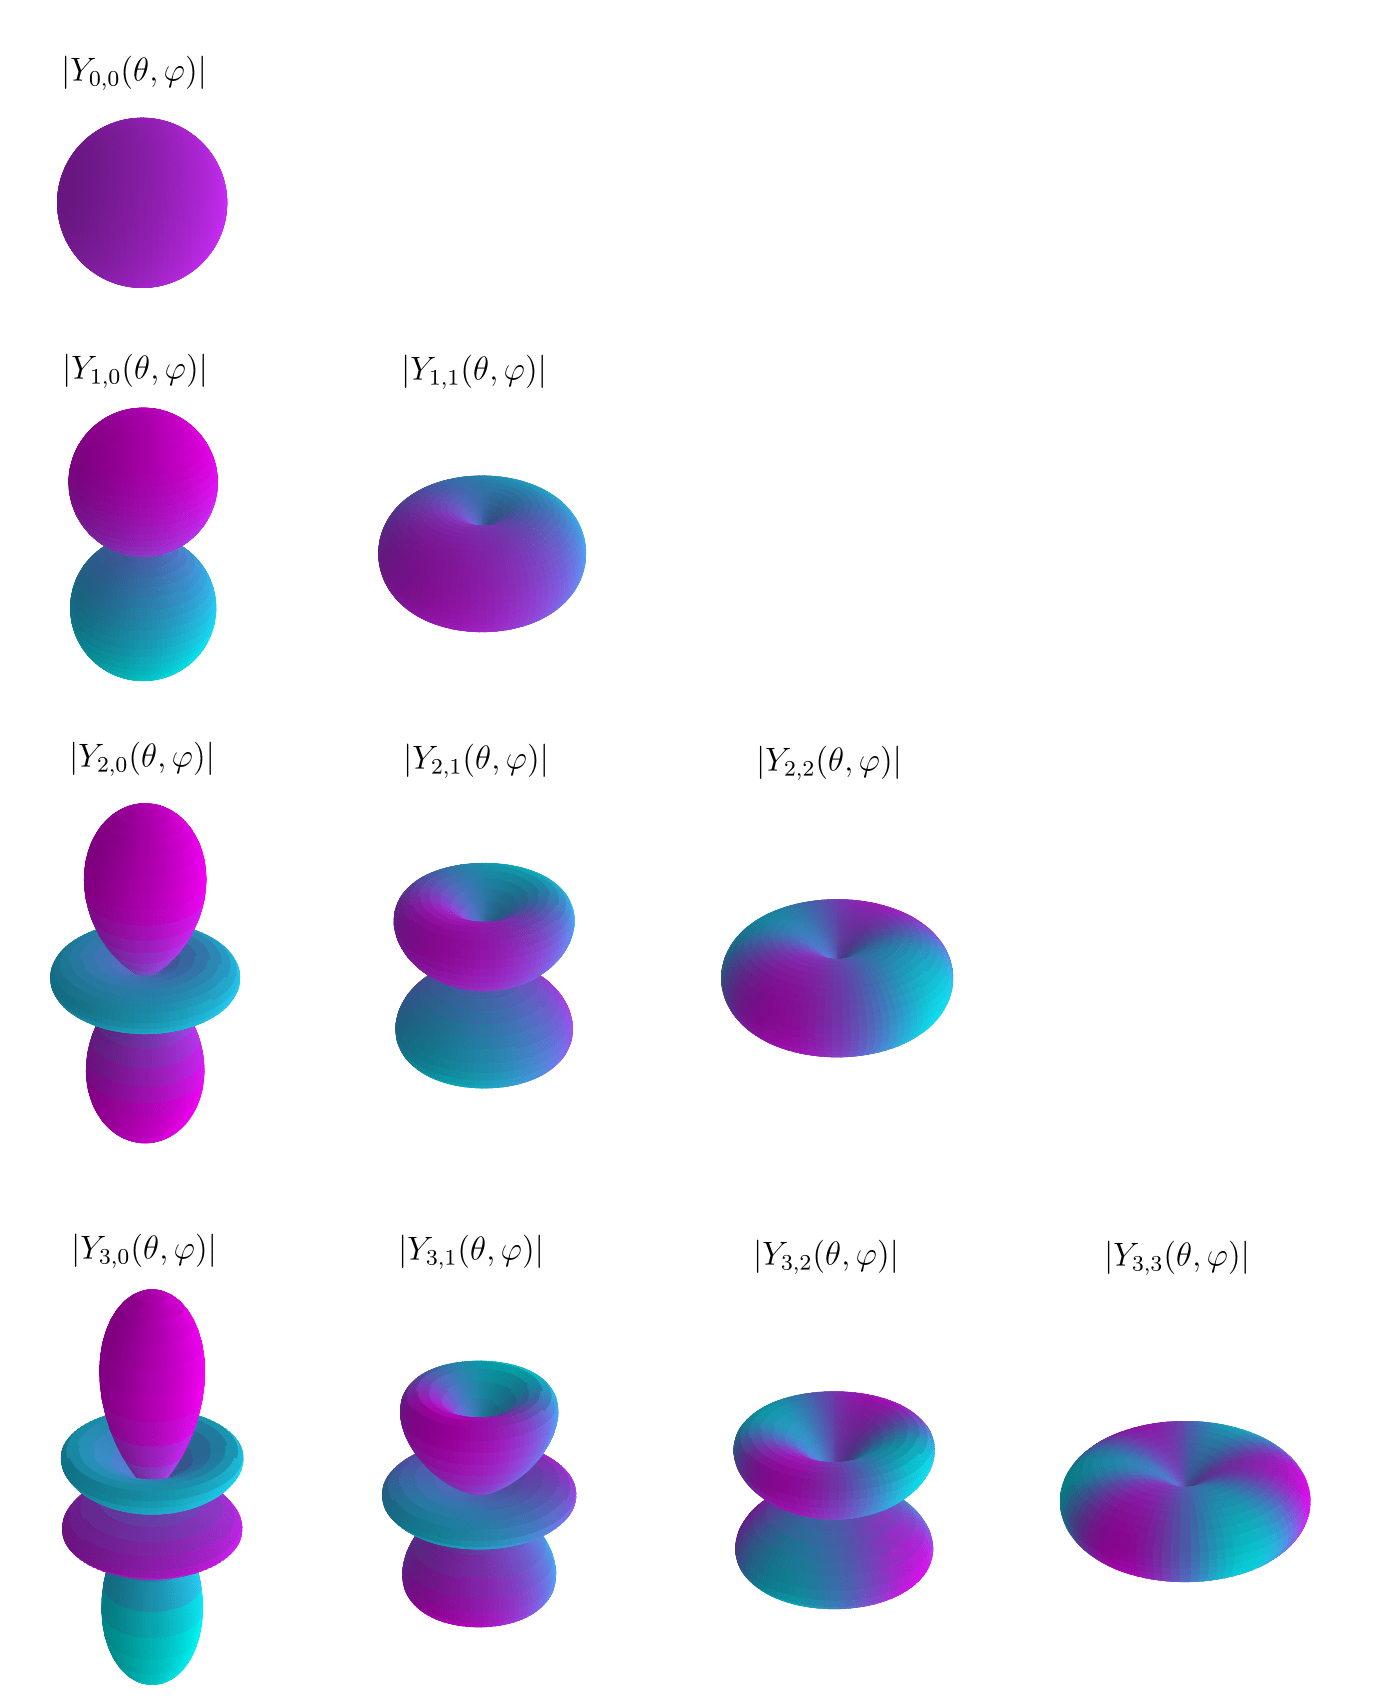
\includegraphics[width=120mm]{../fig/legendre/Ylm.png}
  \caption{球面調和関数$Y_{lm} (\theta, \varphi)$。
	角度$(\theta, \varphi)$に対する$|Y_{lm} (\theta, \varphi)|$の値を原点からの距離として表現している}
\end{figure}


\subsubsection*{証明}

\paragraph{\eqref{eq:Ylm-def-1} $\Longrightarrow$ \eqref{eq:Ylm-def-2}}

\ 
\eqref{eq:Ylm-def-1}をLegendre陪関数の対称性\eqref{eq:Pnm-cos-sym}を用いて書き換えると
\begin{align}
  Y_{lm} (\theta, \varphi)
	&= (-1)^m \sqrt{\frac{2l+1}{4\pi} \frac{(l-m)!}{(l+m)!}} 
		\ (-1)^m\frac{(l+m)!}{(l-m)!} P_l^{-m}(\cos\theta) \, e^{im\varphi} \notag\\
	&= \sqrt{\frac{2l+1}{4\pi} \frac{(l+m)!}{(l-m)!}} 
		\ P_l^{-m}(\cos\theta) \, e^{im\varphi} \label{eq:Ylm-def1->def2}
\end{align}
\eqref{eq:Ylm-def-1}と\eqref{eq:Ylm-def1->def2}はともに
任意の$m \ (-l \leq m \leq l)$について成り立つ式である。
そこで$m \geq 0$のときは\eqref{eq:Ylm-def-1}を、
$m \leq 0$のときは\eqref{eq:Ylm-def1->def2}を用いるという規則を設けることにすると、$Y_{lm}(\theta, \varphi)$は
\begin{equation*}
 Y_{lm}(\theta, \varphi) 
	= (-1)^{\frac{m+|m|}{2}} \sqrt{\frac{2l+1}{4\pi} \frac{(l-|m|)!}{(l+|m|)!}} 
		\ P_l^{|m|}(\cos\theta) \, e^{im\varphi}
\end{equation*}
とかけることが分かる
\footnote{
一般に
\begin{equation*}
  |m| = \left\{
  \begin{alignedat}{2}
    &m &\qquad	& (m\geq 0) \\
    &-m & 		& (m \leq 0)	
  \end{alignedat}
  \right.
\end{equation*}
と書けることに注意せよ。
}
。\qed


\paragraph{定義 $\Longrightarrow$ 偶奇性}
定義\eqref{eq:Ylm-def-1}より
\begin{align*}
  Y_{lm}(\pi-\theta, \varphi+\pi) 
	&= (-1)^m \sqrt{\frac{2l+1}{4\pi} \frac{(l-m)!}{(l+m)!}} 
		\ P_l^m(\cos(\pi-\theta)) \, e^{im(\varphi+\pi)} \notag\\
	&= (-1)^m \sqrt{\frac{2l+1}{4\pi} \frac{(l-m)!}{(l+m)!}} 
		\ P_l^m(-\cos\theta) \cdot (-1)^m e^{im\varphi} \notag\\
	&=  (-1)^l \cdot (-1)^m \sqrt{\frac{2l+1}{4\pi} \frac{(l-m)!}{(l+m)!}} 
		\ P_l^m(\cos\theta) \, e^{im\varphi} \qquad (\since \eqref{eq:Pnm-cos-parity})\notag\\
	&= (-1)^l \ Y_{lm} (\theta, \varphi)
\end{align*}\qed

\paragraph{定義 $\Longrightarrow$ 対称性}
定義\eqref{eq:Ylm-def-1}より
\begin{align*}
  Y_{l, -m} (\theta, \varphi) 
	&= (-1)^{-m} \sqrt{\frac{2l+1}{4\pi} \frac{(l+m)!}{(l-m)!}} 
		\ P_l^{-m} (\cos\theta) \, e^{-im\varphi} \notag\\
	&= (-1)^{-m} \sqrt{\frac{2l+1}{4\pi} \frac{(l+m)!}{(l-m)!}} \cdot
		(-1)^m \frac{(l-m)!}{(l+m)!}P_l^m (\cos\theta) \, e^{-im\varphi} 
		\qquad (\since \eqref{eq:Pnm-cos-sym}) \notag\\
	&= (-1)^m \cdot (-1)^m \sqrt{\frac{2l+1}{4\pi} \frac{(l-m)!}{(l+m)!}}
		\ P_l^m (\cos\theta) \, e^{-im\varphi} \notag\\
	&= (-1)^m \ Y_{lm}(\theta, \varphi)^*
\end{align*}\qed


\paragraph{定義 $\Longrightarrow$ 上昇演算子}
定義\eqref{eq:Ylm-def-1}より
\begin{align*}
  &\hspace{-24pt}e^{i\varphi} \( \frac{\6}{\6\theta} + i \cot\theta\frac{\6}{\6\varphi} \) 
		Y_{lm} (\theta, \varphi) \notag\\
	&= e^{i\varphi} \( \frac{\6}{\6\theta} + i \cot\theta\frac{\6}{\6\varphi} \) 
		(-1)^m \sqrt{\frac{2l+1}{4\pi} \frac{(l-m)!}{(l+m)!}} \ P_l^m(\cos\theta) \, e^{im\varphi} \notag\\
	&= \( \frac{\6}{\6\theta} -m\cot\theta \) 
		(-1)^m \sqrt{\frac{2l+1}{4\pi} \frac{(l-m)!}{(l+m)!}} \ P_l^m(\cos\theta) \, e^{i(m+1)\varphi} 
		\notag\\
	&\, \downarrow \quad  P_n^m (\cos\theta)の上昇演算子\eqref{eq:Pnm-cos-josho} \notag\\
	&= (-1)^{m+1} \sqrt{\frac{2l+1}{4\pi} \frac{(l-m)!}{(l+m)!}} \ P_l^{m+1}(\cos\theta) \, e^{i(m+1)\varphi} 
		\notag\\
	&= \sqrt{(l-m) (l+m+1)} \cdot  (-1)^{m+1} \sqrt{\frac{2l+1}{4\pi} \frac{(l-m-1)!}{(l+m+1)!}} 
		\ P_l^{m+1}(\cos\theta) \, e^{i(m+1)\varphi} \notag\\
	&= \sqrt{(l-m)(l+m+1)} \ Y_{l, m+1} (\theta, \varphi) 
\end{align*}\qed


\paragraph{定義 $\Longrightarrow$ 下降演算子}
定義\eqref{eq:Ylm-def-1}より
\begin{align*}
  &\hspace{-24pt} e^{-i\varphi} \( -\frac{\6}{\6\theta} + i \cot\theta\frac{\6}{\6\varphi} \) 
		Y_{lm} (\theta, \varphi) \notag\\
	&= e^{-i\varphi} \( -\frac{\6}{\6\theta} + i \cot\theta\frac{\6}{\6\varphi} \) 
		(-1)^m \sqrt{\frac{2l+1}{4\pi} \frac{(l-m)!}{(l+m)!}} \ P_l^m(\cos\theta) \, e^{im\varphi} \notag\\
	&= \( -\frac{\6}{\6\theta} -m\cot\theta\frac{\6}{\6\varphi} \) 
		(-1)^m \sqrt{\frac{2l+1}{4\pi} \frac{(l-m)!}{(l+m)!}} \ P_l^m(\cos\theta) \, e^{i(m-1)\varphi} \notag\\
	&\, \downarrow \quad  P_n^m (\cos\theta)の下降演算子\eqref{eq:Pnm-cos-kako} \notag\\
	&= (l+m)(l-m+1) \cdot (-1)^{m-1}  \sqrt{\frac{2l+1}{4\pi} \frac{(l-m)!}{(l+m)!}} 
		\ P_l^{m-1}(\cos\theta) \, e^{i(m-1)\varphi} \notag\\
	&= \sqrt{(l+m)(l-m+1)} \cdot (-1)^{m-1} \sqrt{\frac{2l+1}{4\pi} \frac{(l-m+1)!}{(l+m-1)!}} 
		\ P_l^{m-1}(\cos\theta) \, e^{i(m-1)\varphi} \notag\\
	&= \sqrt{(l+m)(l-m+1)} \ Y_{l, m-1} (\theta, \varphi)
\end{align*}\qed

\paragraph{定義 $\Longrightarrow$ 微分方程式}
まず\eqref{eq:Ylm-diff-eq-1}に定義\eqref{eq:Ylm-def-1}を代入して
先に$\varphi$の微分を実行すると、
$P_n^m (\cos\theta)$の微分方程式\eqref{eq:Pnm-cos-self}とまったく同じ形の式が現れるので、
\eqref{eq:Ylm-diff-eq-1}が成立することが確認できる。
同様に\eqref{eq:Ylm-diff-eq-2}にも定義\eqref{eq:Ylm-def-1}を代入して
$\varphi$の微分を実行することで、その成立を確かめることができる。\qed

\vspace{12pt}
\paragraph{直交性}  $P_n^m(\cos\theta)$の直交性\eqref{eq:Pnm-cos-chokko}および
$e^{im\varphi}$の直交性により直ちに示される。\qed


\subsection{量子力学への応用}

\subsubsection{軌道}
表\ref{tab:Ylm}からも分かるように、一般に球面調和関数は複素関数であり、
その視覚的なイメージがつかみにくくなっている。
そこで球面調和関数同士で適当な線形結合を行うことで実関数をつくり、
方向性などが読み取りやすい形に書き直すことがある。
このようにして考えられる関数は\textbf{軌道}と呼ばれ、量子化学などの分野で広く扱われる。
表\ref{tab:orbital}に軌道の具体的な定義および表式
\footnote{
軌道の表記は文献によりまちまちである。
たとえば$d_{z^2}$軌道は$d_{3z^2-r^2}$軌道と書かれることも多い。
}
、
図\ref{tab:orbital}に角$(\theta, \varphi)$における軌道の絶対値を原点からの距離としてプロットしたものを示す。

% $を何度も書くのに嫌気が差したので
%\begin{table}[ptb]
%  \centering
%  \caption{軌道}
%  \begin{tabular}{c|c|lll}\Hline
%    & & \multicolumn{3}{c}{} \\\hline
%    $s$ & $s$ & $Y_{00}$ & $\sqrt{\frac{1}{4\pi}}$ & \\\hdashline
%    & $p_x$ & $\frac{1}{\sqrt{2}} (-Y_{11}+Y_{1, -1})$ & $\sqrt{\frac{3}{4\pi}}\sin\theta\cos\varphi$ & 
%		$\sqrt{\frac{3}{4\pi}}\frac{x}{r}$ \\
%    $p$ & $p_y$ & $-\frac{1}{\sqrt{2}i} (Y_{11} + Y_{1, -1})$ & $\sqrt{\frac{3}{4\pi}}\sin\theta\sin\varphi$ &
%    $\sqrt{\frac{3}{4\pi}} \frac{y}{r}$ \\
%    & $p_z$ & $Y_{10}$ & $\sqrt{\frac{3}{4\pi}}\cos\theta$ & $\sqrt{\frac{3}{4\pi}} \frac{z}{r}$ \\\hdashline
%    & $d_{xy}$ & $\frac{1}{\sqrt{2} i} (Y_{22} - Y_{2,-2})$ 
%	& $\sqrt{\frac{15}{4\pi}} \sin^2\theta\sin\varphi\cos\varphi$ & $\sqrt{\frac{15}{4\pi}}\frac{xy}{r^2}$ \\
%  \end{tabular}
%\end{table}

\begin{table}[ptb]
  \centering\small
  \caption{軌道の定義式および具体的な表式}
  \label{tab:orbital}
  $\begin{array}{c|c|lll}\Hline
    & & \multicolumn{3}{c}{} \\\hline
    s & s & Y_{00} & \sqrt{\frac{1}{4\pi}} & \sqrt{\frac{1}{4\pi}} \\\hdashline
    & p_y & -\frac{1}{\sqrt{2}i} (Y_{11} + Y_{1, -1}) & \sqrt{\frac{3}{4\pi}}\sin\theta\sin\varphi &
    \sqrt{\frac{3}{4\pi}} \frac{y}{r} \\
    p & p_z & Y_{10} & \sqrt{\frac{3}{4\pi}}\cos\theta & \sqrt{\frac{3}{4\pi}} \frac{z}{r} \\
    & p_x & \frac{1}{\sqrt{2}} (-Y_{11}+Y_{1, -1}) & \sqrt{\frac{3}{4\pi}}\sin\theta\cos\varphi & 
		\sqrt{\frac{3}{4\pi}}\frac{x}{r} \\\hdashline
    & d_{xy} & \frac{1}{\sqrt{2} i} (Y_{22} - Y_{2,-2}) 
	& \sqrt{\frac{15}{4\pi}} \sin^2\theta\sin\varphi\cos\varphi & \sqrt{\frac{15}{4\pi}}\frac{xy}{r^2} \\
    & d_{yz} & -\frac{1}{\sqrt{2} i} (Y_{21} + Y_{2,-1})
	& \sqrt{\frac{15}{4\pi}} \cos\theta\sin\theta\sin\varphi & \sqrt{\frac{15}{4\pi}}\frac{yz}{r^2} \\
    d& d_{z^2} & Y_{20}
	& \sqrt{\frac{5}{16\pi}} (3\cos^2\theta-1) & \sqrt{\frac{5}{16\pi}}\frac{3z^2-r^2}{r^2} \\
    & d_{zx} & -\frac{1}{\sqrt{2}} (Y_{21} - Y_{2,-1})
	& \sqrt{\frac{15}{4\pi}} \cos\theta\sin\theta\cos\varphi & \sqrt{\frac{15}{4\pi}}\frac{zx}{r^2} \\
    & d_{x^2-y^2} & \frac{1}{\sqrt{2}} (Y_{22} + Y_{2,-2})
	& \sqrt{\frac{15}{16\pi}} \sin^2\theta(\cos^2\varphi-\sin^2\varphi) 
	& \sqrt{\frac{15}{16\pi}}\frac{x^2-y^2}{r^2} \\\hdashline
    & f_{y(3x^2-y^2)} & -\frac{1}{\sqrt{2} i} (Y_{33} + Y_{3,-3})
	& \sqrt{\frac{35}{32\pi}} \sin^3\theta\sin\varphi(3\cos^2\varphi-\sin^2\varphi) 
	& \sqrt{\frac{35}{32\pi}}\frac{y(3x^2-y^2)}{r^3} \\
    & f_{xyz} & \frac{1}{\sqrt{2} i} (Y_{32} - Y_{3,-2})
	& \sqrt{\frac{105}{4\pi}} \cos\theta\sin^2\theta\cos\varphi\sin\varphi 
	& \sqrt{\frac{105}{4\pi}}\frac{xyz}{r^3} \\
    & f_{yz^2} & -\frac{1}{\sqrt{2} i} (Y_{31} + Y_{3,-1})
	& \sqrt{\frac{21}{32\pi}} \sin\theta\sin\varphi(5\cos^2\theta-1) 
	& \sqrt{\frac{21}{32\pi}}\frac{y(5z^2-r^2)}{r^3} \\
    f& f_{z^3} & Y_{30}
	& \sqrt{\frac{7}{16\pi}} \cos\theta(5\cos^2\theta-3) 
	& \sqrt{\frac{7}{16\pi}}\frac{z(5z^2-3r^2)}{r^3} \\
    & f_{xz^2} & -\frac{1}{\sqrt{2}} (Y_{31} - Y_{3,-1})
	& \sqrt{\frac{21}{32\pi}} \sin\theta\cos\varphi (5\cos^2\theta-1) 
	& \sqrt{\frac{21}{32\pi}}\frac{x(5z^2-r^2)}{r^3} \\
    & f_{z(x^2-y^2)} & \frac{1}{\sqrt{2}} (Y_{32} + Y_{3,-2})
	& \sqrt{\frac{105}{16\pi}} \cos\theta\sin^2\theta (\cos^2\varphi-\sin^2\varphi) 
	& \sqrt{\frac{105}{16\pi}}\frac{z(x^2-y^2)}{r^3} \\
    & f_{x(x^2-3y^2)} & -\frac{1}{\sqrt{2}} (Y_{33} - Y_{3,-3})
	& \sqrt{\frac{35}{32\pi}} \sin^3\theta\cos\varphi(\cos^2\varphi-3\sin^2\varphi) 
	& \sqrt{\frac{35}{32\pi}}\frac{x(x^2-3y^2)}{r^3} \\\hline
  \end{array}$
\end{table}

\begin{figure}[tbp]
  \centering
  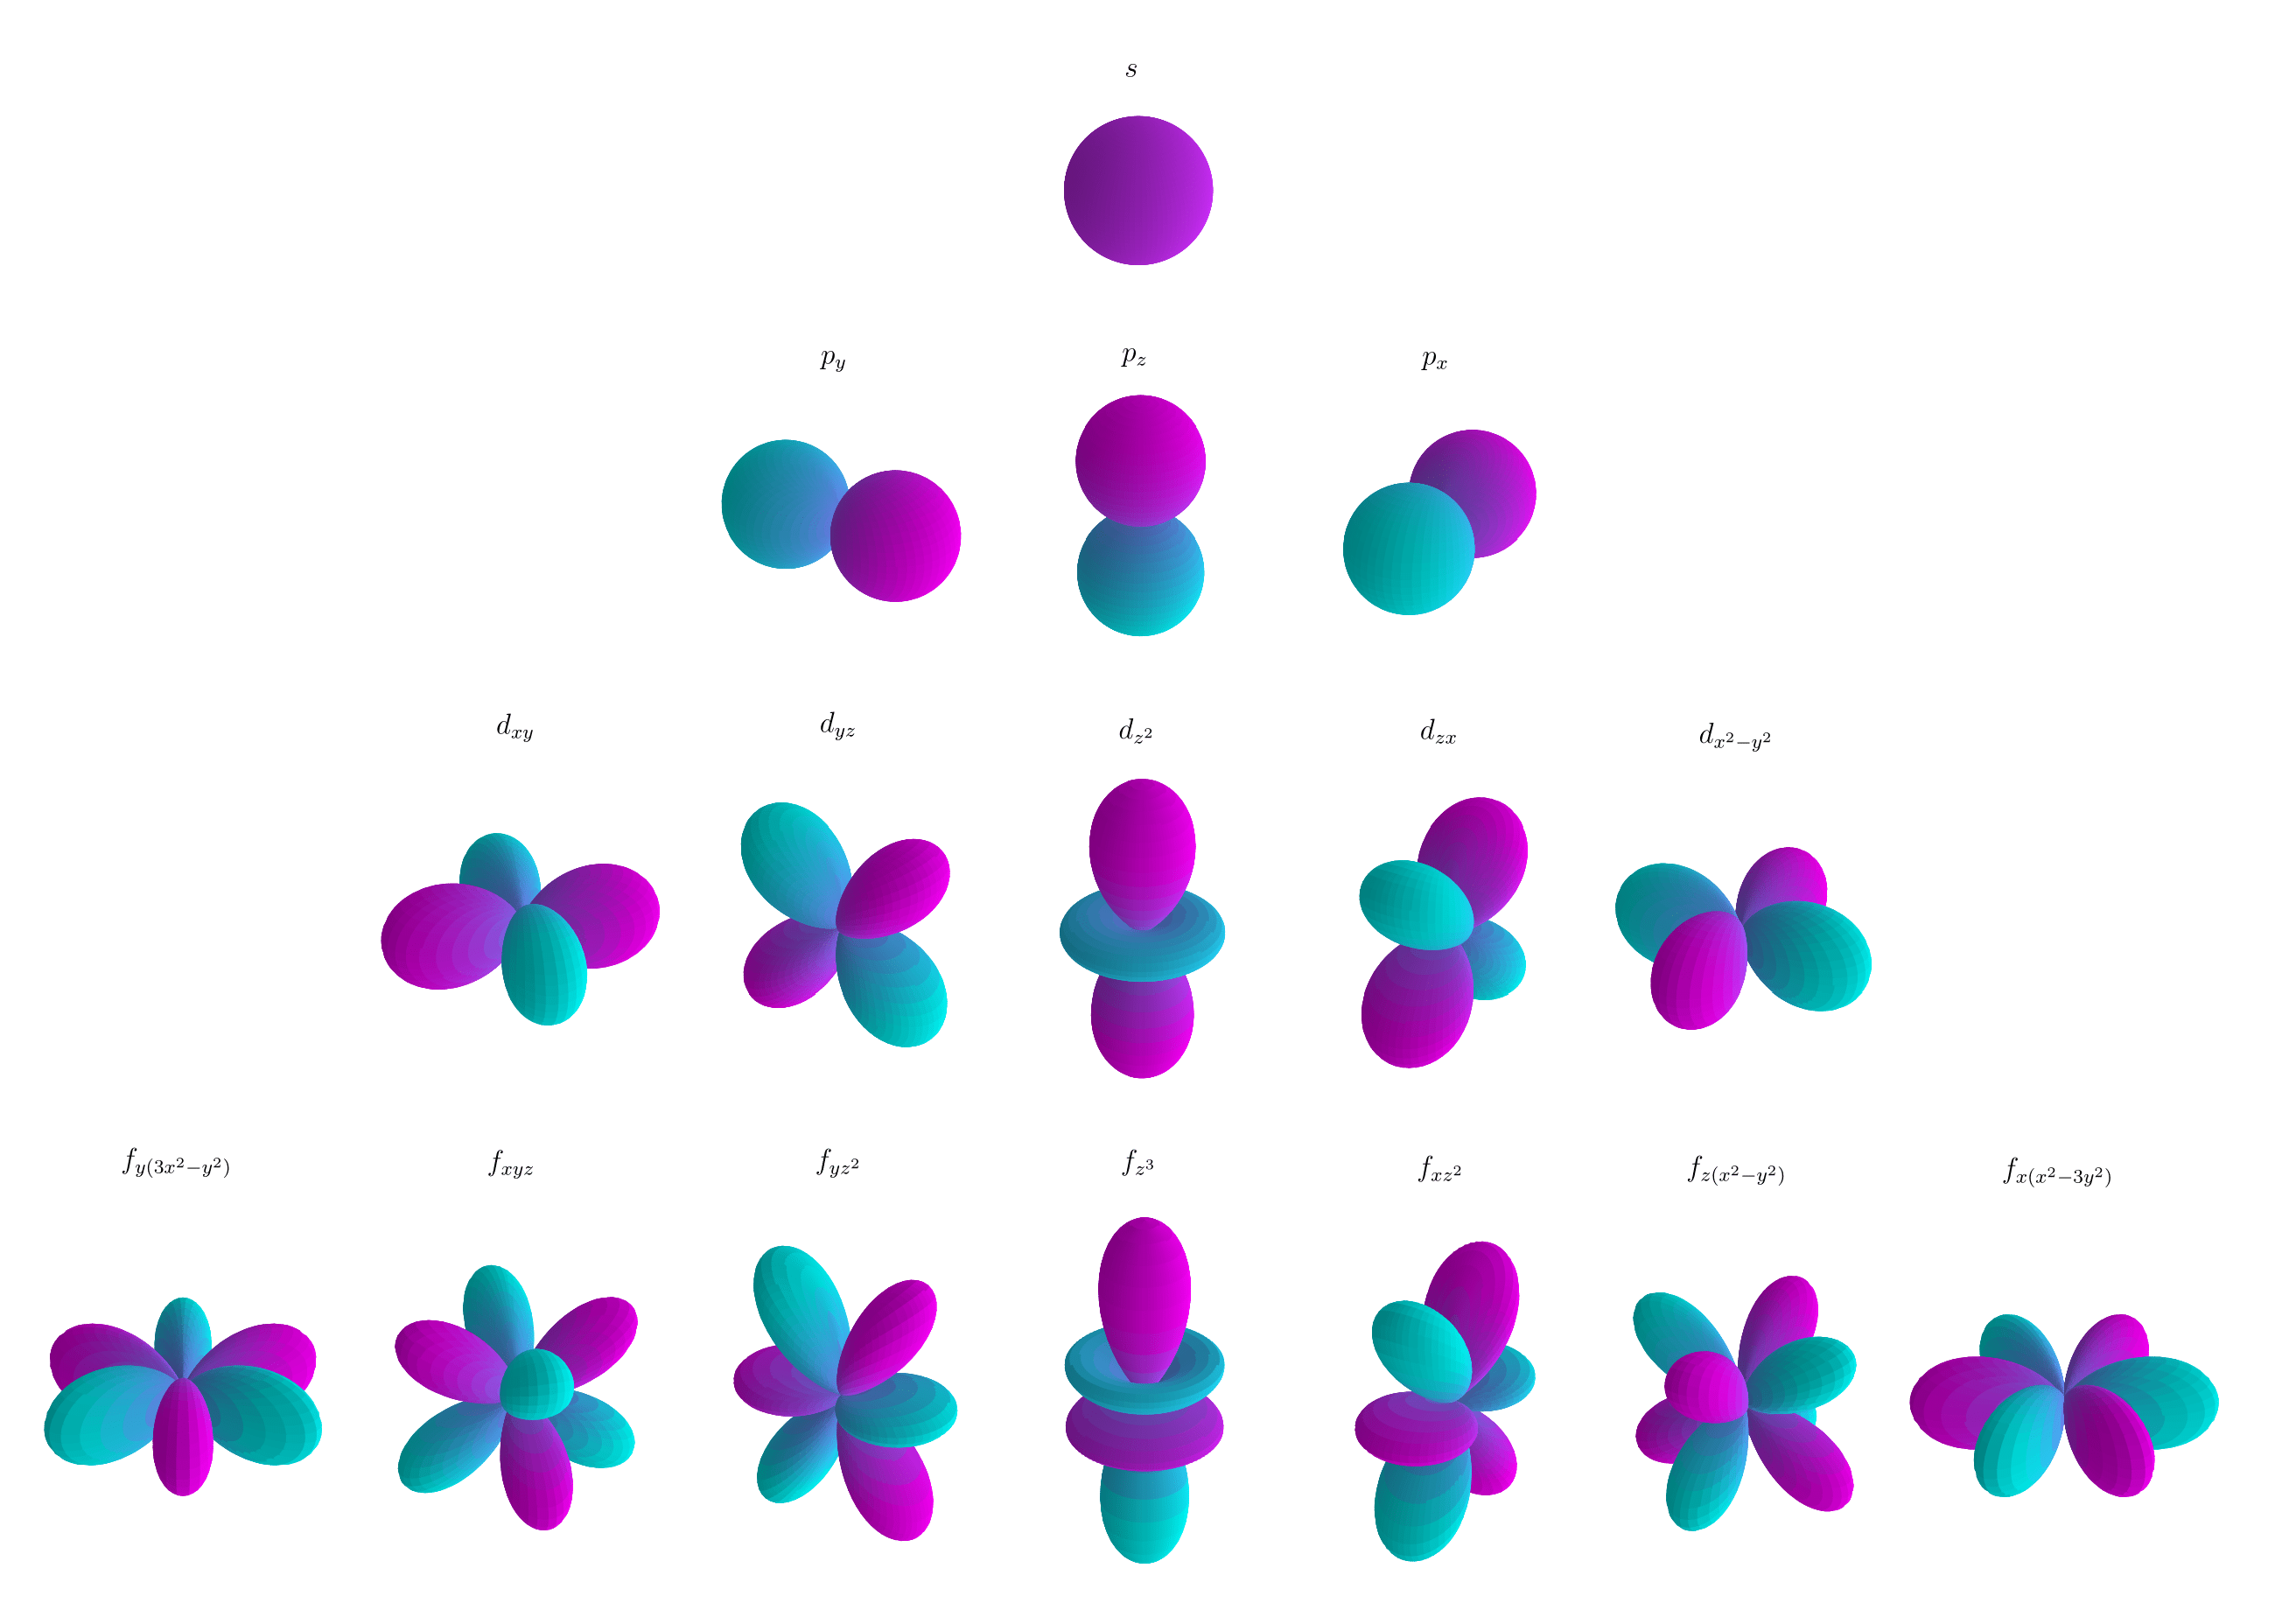
\includegraphics[width=150mm]{../fig/legendre/orbital.png}
  \caption{軌道。角$(\theta, \varphi)$における軌道の絶対値を原点からの距離として表現している。
	なお紫色の部分は正、水色の部分は負であることを表す}
  \label{fig:orbital}
\end{figure}

\subsubsection{軌道角運動量}
量子力学において、軌道角運動量演算子$\hat{\bm{L}} = (\hat{L}_x, \hat{L}_y, \hat{L}_z)$は
位置座標演算子$\hat{\bm{r}} = (\hat{x}, \hat{y}, \hat{z}) = (x, y, z)$および
運動量演算子$\hat{\bm{p}} = (\hat{p}_x, \hat{p}_y, \hat{p}_z)  = -i\hbar \nabla$によって
\begin{equation}
  \hat{\bm{L}} = \hat{\bm{r}} \times \hat{\bm{p}}
\end{equation}
と定義される。成分に分けて書くと
\begin{align*}
  \hat{L}_x &=\hat{y} \hat{p}_z - \hat{z} \hat{p}_y  
		= -i\hbar \( y \frac{\6}{\6 z} - z \frac{\6}{\6 y} \) \\
  \hat{L}_y &=\hat{z} \hat{p}_x - \hat{x} \hat{p}_z  
		= -i\hbar \( z \frac{\6}{\6 x} - x \frac{\6}{\6 z} \) \\
  \hat{L}_z &=\hat{x} \hat{p}_y - \hat{y} \hat{p}_x  
		= -i\hbar \( x \frac{\6}{\6 y} - y \frac{\6}{\6 x} \)
\end{align*}
である。
これらを球座標$(r, \theta, \varphi)$で表すと、少し長い計算を経て
\begin{align}
  \hat{L}_x &= -i\hbar \( -\sin\varphi \frac{\6}{\6\theta} 
		- \cot\theta \cos\varphi \frac{\6}{\6\varphi} \) \\
  \hat{L}_y &= -i\hbar \( \cos\varphi \frac{\6}{\6 \theta}
		- \cot\theta \sin\varphi \frac{\6}{\6\varphi} \) \\
  \hat{L}_z &= -i\hbar \frac{\6}{\6\varphi} \label{eq:Lz}
\end{align}
となる。
そして角運動量の2乗$\hat{\bm{L}}^2$を$\hat{L}_x^2 + \hat{L}_y^2 + \hat{L}_z^2$によって定義すると、
さらに長々しい計算を経て
\begin{equation}\label{eq:L^2}
  \hat{\bm{L}}^2
	= -\hbar^2 \[ \frac{1}{\sin\theta} \frac{\6}{\6\theta} \( \sin\theta \frac{\6}{\6\theta} \)
	+ \frac{1}{\sin^2\theta} \frac{\6^2}{\6 \varphi^2} \] 
\end{equation}
が得られる。

ここで球面調和関数の微分方程式\eqref{eq:Ylm-diff-eq-1}, \eqref{eq:Ylm-diff-eq-2}と
角運動量の$2$乗\eqref{eq:L^2}, $z$成分\eqref{eq:Lz}を見比べてみると
まったく同じ形が現れていることが分かる。
これより、$\hat{\bm{L}}^2, \ \hat{L}_z$と球面調和関数$Y_{lm} (\theta, \varphi)$の間には
\begin{align}
  \hat{\bm{L}}^2 \, Y_{lm} (\theta, \varphi)
	&= l(l+1) \hbar^2 \ Y_{lm} (\theta, \varphi) \label{eq:eigen1}\\
  \hat{L}_z \, Y_{lm} (\theta, \varphi)
	&= m\hbar \ Y_{lm} (\theta, \varphi) \label{eq:eigen2}
\end{align} 
という関係が成り立つ。
\eqref{eq:eigen1}, \eqref{eq:eigen2}は、球面調和関数$Y_{lm} (\theta, \varphi)$が
$\hat{\bm{L}}^2$と$\ \hat{L}_z$の同時固有関数であり、
固有値がそれぞれ$ l(l+1) \hbar^2, m\hbar$であることを表している。
これは中心力場のSchr\"{o}dinger方程式を議論する際に現れる。

また、軌道角運動量の昇降演算子は次のように定義される。
\begin{alignat}{2}
  &\textbf{上昇演算子} & \quad &\hat{L}_{+} = \hat{L}_x + i \hat{L}_y 
	= \hbar e^{i\varphi} \( \frac{\6}{\6\theta} + i\cot \frac{\6}{\6\varphi} \) \\
  &\textbf{下降演算子} & \quad &\hat{L}_{-} = \hat{L}_x - i \hat{L}_y 
	= \hbar e^{-i\varphi} \( -\frac{\6}{\6\theta} + i\cot \frac{\6}{\6\varphi} \)
\end{alignat}
これらと球面調和関数の昇降演算子\eqref{eq:Ylm-josho}, \eqref{eq:Ylm-kako}とを比べると、
やはり同じ形が現れている。
すなわち、軌道角運動量の昇降演算子と球面調和関数の間には次のような関係が成り立つことになる。
\begin{align}
  \hat{L}_{+} Y_{l, m} (\theta, \varphi) &= \sqrt{(l-m)(l+m+1)} \, \hbar \ Y_{l, m+1} (\theta, \varphi) \\
  \hat{L}_{-} Y_{l, m} (\theta, \varphi) &= \sqrt{(l+m)(l-m+1)} \, \hbar \ Y_{l, m-1} (\theta, \varphi)
\end{align}
このように、球面調和関数は量子力学で議論される角運動量を理解するうえで重要な役割を果たす。


\end{document}